%!TeX spellcheck = en-US
\documentclass{beamer}
\usepackage[utf8]{inputenc}
\usepackage{amsmath}
\usepackage{amsthm}
% \usepackage{algorithm}
% \usepackage{algorithmic}
% !TEX root = neurips_2019.tex
% !TeX spellcheck = en-US
\usepackage{times,wrapfig,amsmath,amsfonts,bm,color,enumitem,algorithm,algpseudocode}

\usepackage{times}
\usepackage{amsmath,amssymb,amsthm,bbm,mathtools}
\usepackage{graphicx}
\usepackage{subfigure}
\usepackage{hyperref}
\usepackage{url}
\usepackage{pbox}

\newcommand\tTab{\rule{0pt}{2.5ex}}       % Top strut
\newcommand\bTab{\rule[-1.5ex]{0pt}{0pt}} % Bottom strut

\newcommand{\w}{\ensuremath{\mathbf{w}}}
\newcommand{\W}{\ensuremath{\mathbf{W}}}
\renewcommand{\u}{\ensuremath{\mathbf{u}}}
\renewcommand{\v}{\ensuremath{\mathbf{v}}}
\newcommand{\x}{\ensuremath{\mathbf{x}}}
\newcommand{\half}{\frac{1}{2}}
\newcommand{\argmin}[1]{\underset{#1}{\mathrm{argmin}} \:}
\newcommand{\argmax}[1]{\underset{#1}{\mathrm{argmax}} \:}
\newcommand{\inner}[2]{\left\langle #1, #2 \right\rangle}
\newcommand{\gb}[1]{\boldsymbol{#1}}
\newcommand{\hinge}[1]{\left[#1\right]_+}

\newcommand{\valpha}{\gb{\alpha}}
\newcommand{\vtheta}{\gb{\theta}}
\newcommand{\vmu}{\gb{\mu}}
\newcommand{\vnu}{\gb{\nu}}
\newcommand{\D}{\mathcal{D}}
\newcommand{\proj}{P}
\newcommand{\hbeta}{\hat{\beta}}

\newcommand{\lnd}[1]{\ln\left(\frac{#1}{\delta}\right)}
\newcommand{\slnd}[1]{\ln({#1}/{\delta})}

\newcommand{\one}[1]{\left[\!\left[ #1 \right]\!\right]}
\newcommand{\ones}{\mathbbm{1}}
\newcommand{\E}{\ensuremath{\mathbbf{E}}}
\renewcommand{\P}{\ensuremath{\mathbb{P}}}

\newcommand{\etal}{{\it et al}}

\newcommand{\norm}[1]{\left\lVert{#1}\right\rVert}
\newcommand{\abs}[1]{\left\lvert{#1}\right\rvert}
\newcommand{\vnorm}[1]{\left\lVert{#1}\right\rVert} % vector norm
\newcommand{\mnorm}[1]{\left\lVert{#1}\right\rVert} % matrix norm
\newcommand{\loss}[2]{\ell({#1};{#2})}
\newcommand{\regzr}[1]{R({#1})} % regularizer
\newcommand{\generr}[1]{\ell({#1})} % generalization error of a predictor
\newcommand{\emperr}[1]{{\hat{\ell}}({#1})}

\newcommand{\wml}{\hat{w}} % w minimizing training regularized objective
\newcommand{\waprox}{w^*} % w minimizing regularized gen error
\newcommand{\walg}{\tilde{w}} % output of algorithm

\newcommand{\optacc}{\epsilon_{\text{acc}}}
\newcommand{\apperr}{\epsilon_{\text{aprx}}}
\newcommand{\esterr}{\epsilon_{\text{est}}}
\newcommand{\opterr}{\epsilon_{\text{opt}}}

\newcommand{\rank}{\operatorname{rank}}
\newcommand{\diag}{\operatorname{diag}}
\newcommand{\trace}{\operatorname{trace}}
\newcommand{\sign}{\operatorname{sign}}
\newcommand{\conv}{\operatorname{conv}}

\newcommand{\R}{\mathbb{R}}
\newcommand{\C}{\mathbb{C}}
\newcommand{\Z}{\mathbb{Z}}

\newcommand{\FF}{\mathcal{F}}
\newcommand{\HH}{\mathcal{H}}
\newcommand{\GG}{\mathcal{G}}

\newcommand{\ceil}[1]{\lceil #1\rceil}
\newcommand{\floor}[1]{\lfloor #1\rfloor}

\newcommand{\mip}[2]{{\left\langle{#1},{#2}\right\rangle}}


\newcommand{\defeq}{\triangleq}


\mathchardef\hyphen="2D

\usepackage{times}
\usepackage{amsmath,amssymb,amsthm}
\usepackage{graphicx}
\usepackage{subfigure}
\usepackage{hyperref}
\usepackage{url}
\usepackage{pbox}

\newcommand{\T}{^\top}
\newcommand{\TT}{\top }
\newcommand{\RR}{\mathbb{R}}
\newcommand{\EE}{\mathbb{E}}
\newcommand{\MM}{\mathcal{M}}

% \newtheorem{thm}{Theorem}
% \newtheorem{lem}{Lemma}
\newtheorem{cor}{Corollary}
% \newtheorem{Def}{Definition}
% \newtheorem{note}{Note}

\newcommand{\calA}{\mathcal{A}}
\newcommand{\calB}{\mathcal{B}}
\newcommand{\calC}{\mathcal{C}}
\newcommand{\calD}{\mathcal{D}}
\newcommand{\calE}{\mathcal{E}}
\newcommand{\calF}{\mathcal{F}}
\newcommand{\calG}{\mathcal{G}}
\newcommand{\calH}{\mathcal{H}}
\newcommand{\calI}{\mathcal{I}}
\newcommand{\calJ}{\mathcal{J}}
\newcommand{\calK}{\mathcal{K}}
\newcommand{\calL}{\mathcal{L}}
\newcommand{\calM}{\mathcal{M}}
\newcommand{\calN}{\mathcal{N}}
\newcommand{\calO}{\mathcal{O}}
\newcommand{\calP}{\mathcal{P}}
\newcommand{\calQ}{\mathcal{Q}}
\newcommand{\calR}{\mathcal{R}}
\newcommand{\calS}{\mathcal{S}}
\newcommand{\calT}{\mathcal{T}}
\newcommand{\calU}{\mathcal{U}}
\newcommand{\calV}{\mathcal{V}}
\newcommand{\calW}{\mathcal{W}}
\newcommand{\calX}{\mathcal{X}}
\newcommand{\calY}{\mathcal{Y}}
\newcommand{\calZ}{\mathcal{Z}}

\newcommand{\mathA}{\mathbb{A}}
\newcommand{\mathB}{\mathbb{B}}
\newcommand{\mathC}{\mathbb{C}}
\newcommand{\mathD}{\mathbb{D}}
\newcommand{\mathE}{\mathbb{E}}
\newcommand{\mathF}{\mathbb{F}}
\newcommand{\mathG}{\mathbb{G}}
\newcommand{\mathH}{\mathbb{H}}
\newcommand{\mathI}{\mathbb{I}}
\newcommand{\mathJ}{\mathbb{J}}
\newcommand{\mathK}{\mathbb{K}}
\newcommand{\mathL}{\mathbb{L}}
\newcommand{\mathM}{\mathbb{M}}
\newcommand{\mathN}{\mathbb{N}}
\newcommand{\mathO}{\mathbb{O}}
\newcommand{\mathP}{\mathbb{P}}
\newcommand{\mathQ}{\mathbb{Q}}
\newcommand{\mathR}{\mathbb{R}}
\newcommand{\mathS}{\mathbb{S}}
\newcommand{\mathT}{\mathbb{T}}
\newcommand{\mathU}{\mathbb{U}}
\newcommand{\mathV}{\mathbb{V}}
\newcommand{\mathW}{\mathbb{W}}
\newcommand{\mathX}{\mathbb{X}}
\newcommand{\mathY}{\mathbb{Y}}
\newcommand{\mathZ}{\mathbb{Z}}

\newcommand{\veca}{\mathbf{a}}
\newcommand{\vecd}{\mathbf{d}}
\newcommand{\vece}{\mathbf{e}}
\newcommand{\vecf}{\mathbf{f}}
\newcommand{\vecg}{\mathbf{g}}
\newcommand{\vech}{\mathbf{h}}
\newcommand{\veci}{\mathbf{i}}
\newcommand{\vecj}{\mathbf{j}}
\newcommand{\veck}{\mathbf{k}}
\newcommand{\vecl}{\mathbf{l}}
\newcommand{\vecm}{\mathbf{m}}
\newcommand{\vecn}{\mathbf{n}}
\newcommand{\veco}{\mathbf{o}}
\newcommand{\vecp}{\mathbf{p}}
\newcommand{\vecq}{\mathbf{q}}
\newcommand{\vecr}{\mathbf{r}}
\newcommand{\vecs}{\mathbf{s}}
\newcommand{\vect}{\mathbf{t}}
\newcommand{\vecu}{\mathbf{u}}
\newcommand{\vecv}{\mathbf{v}}
\newcommand{\vecw}{\mathbf{w}}
\newcommand{\vecx}{\mathbf{x}}
\newcommand{\vecy}{\mathbf{y}}
\newcommand{\vecz}{\mathbf{z}}

\newcommand{\numinputs}{d}
\newcommand{\numoutputs}{k}
\newcommand{\numhiddens}{H}
\newcommand{\mU}{\boldsymbol{U}}
% \newcommand{\mV}{\boldsymbol{V}}
\newcommand{\mW}{\boldsymbol{W}}
\newcommand{\rect}{\text{rect}}
\newcommand{\gpath}{\text{path}}
\newcommand{\layer}{\text{layer}}
\newcommand{\DAG}{\text{DAG}}
\newcommand{\dout}{d_\text{out}}
\newcommand{\din}{d_\text{in}}
\newcommand{\vin}{v_{\textrm{in}}}
\newcommand{\vout}{v_{\textrm{out}}}
\newcommand{\relu}{\sigma_{\textsc{relu}}}
\newcommand{\gnorm}[1]{\norm{#1}}
\newcommand{\mugeom}{\mu^{\textit{geo}}}
\newcommand{\pathr}{\phi}
\newcommand{\convexnn}{\nu}
\newcommand{\net}{{\rm net}}
\newcommand{\removed}[1]{}
% \newcommand{\fix}{\marginpar{FIX}}
% \newcommand{\new}{\marginpar{NEW}}
\newcommand{\var}{\mathrm{Var}}
\newcommand{\cov}{\mathrm{Cov}}
\newcommand{\In}{\text{in}}
\newcommand{\Out}{\text{out}}
\newcommand{\vecX}{\mathbf{x}}
\newcommand{\vecH}{\mathbf{h}}
\newcommand{\vecW}{\mathbf{w}}
\newcommand{\vecY}{\mathbf{y}}
\renewcommand{\vec}[1]{\mathrm{vec}(#1)}
\newcommand{\vh}{{\vec h}}
\newcommand{\vw}{{\vec w}}
% \newcommand{\vx}{{\vec x}}
\newcommand{\vz}{{\vec z}}
\newcommand{\vphi}{\boldsymbol{\phi}}
\newcommand{\vpi}{\boldsymbol{\pi}}
\newcommand{\vecGam}{\boldsymbol{\gamma}}
\newcommand{\vecDelta}{\boldsymbol{\Delta}}
\newcommand{\vecb}{\vec b}
\newcommand{\vecc}{\vec c}
\newcommand{\tV}{\widetilde{V}}
% \newcommand{\tW}{\widetilde{\vec W}}
\newcommand{\tH}{\widetilde{\vec h}}
\newcommand{\vecmu}{\boldsymbol{\mu}}

\newcommand{\St}{\ensuremath{\mathrm{St}}}
\newcommand{\Ob}{\ensuremath{\mathrm{Ob}}}
\newcommand{\I}{\ensuremath{\mathbf{I}}}
\newcommand{\Exp}{\ensuremath{\mathrm{Exp}}}
\newcommand{\Rt}{\ensuremath{\mathrm{Rt}}}
\newcommand{\tangent}{\ensuremath{\mathit{T}_{\mathbf{W}}\mathcal{M}}}
\DeclareMathOperator{\Tr}{Tr}
\newcommand{\h}{\mathbf{h}}
\newcommand{\J}{\mathbf{J}}
\newcommand{\A}{\mathbf{A}}
\newcommand{\G}{\mathbf{G}}
% \newcommand{\H}{\mathbf{H}}
% \makeatletter
% \def\vec{\mathop{\operator@font vec}\nolimits}
% \makeatother
\newtheorem*{remark}{Remark}
\newtheorem{proposition}{Proposition}
% \newtheorem{theorem}{Theorem}
\newtheorem{assumption}{Assumption}
% \newtheorem*{definition}{Definition}
% \newtheorem{lemma}{Lemma}
\newtheorem{asu}{Assumption}
\newcounter{subassumption}[asu]
\renewcommand{\thesubassumption}{(\textit{\roman{subassumption}})}
\makeatletter
\renewcommand{\p@subassumption}{\theasu}% Counter prefix.
\makeatother
\newcommand{\subasu}{% Just like \item in a list, but for an asu
  \refstepcounter{subassumption}%
  \thesubassumption~\ignorespaces}

% Figure reference, lower-case.
\def\figref#1{figure~\ref{#1}}
% Figure reference, capital. For start of sentence
\def\Figref#1{Figure~\ref{#1}}
\def\twofigref#1#2{figures \ref{#1} and \ref{#2}}
\def\quadfigref#1#2#3#4{figures \ref{#1}, \ref{#2}, \ref{#3} and \ref{#4}}
% Section reference, lower-case.
\def\secref#1{section~\ref{#1}}
% Section reference, capital.
\def\Secref#1{Section~\ref{#1}}
% Reference to two sections.
\def\twosecrefs#1#2{sections \ref{#1} and \ref{#2}}
% Reference to three sections.
\def\secrefs#1#2#3{sections \ref{#1}, \ref{#2} and \ref{#3}}
% Reference to an equation, lower-case.
\def\eqref#1{equation~\ref{#1}}
% Reference to an equation, upper case
\def\Eqref#1{Equation~\ref{#1}}
% A raw reference to an equation---avoid using if possible
\def\plaineqref#1{\ref{#1}}
% Reference to a chapter, lower-case.
\def\chapref#1{chapter~\ref{#1}}
% Reference to an equation, upper case.
\def\Chapref#1{Chapter~\ref{#1}}
% Reference to a range of chapters
\def\rangechapref#1#2{chapters\ref{#1}--\ref{#2}}
% Reference to an algorithm, lower-case.
% \def\algref#1{algorithm~\ref{#1}}
% Reference to an algorithm, upper case.
% \def\Algref#1{Algorithm~\ref{#1}}
% \def\twoalgref#1#2{algorithms \ref{#1} and \ref{#2}}
% \def\Twoalgref#1#2{Algorithms \ref{#1} and \ref{#2}}
% Reference to a part, lower case
% \def\partref#1{part~\ref{#1}}
% Reference to a part, upper case
% \def\Partref#1{Part~\ref{#1}}
% \def\twopartref#1#2{parts \ref{#1} and \ref{#2}}

%% Sets page size and margins
%\usepackage[a4paper,top=3cm,bottom=2cm,left=3cm,right=3cm,marginparwidth=1.75cm]{geometry}
% \DeclareMathOperator*{\argmax}{arg\,max}
% \DeclareMathOperator*{\argmin}{arg\,min}
% \DeclareMathOperator*{\max}{max}
% \DeclareMathOperator*{\min}{min}
\usepackage{graphicx}
\usepackage{amsfonts,amssymb}

\title{Variational Calculus}
\author{}
\date{June 2019}

\begin{document}

\maketitle

\begin{frame}{Intro to infinite-dimensional optimization}
    \begin{figure}
        \centering
        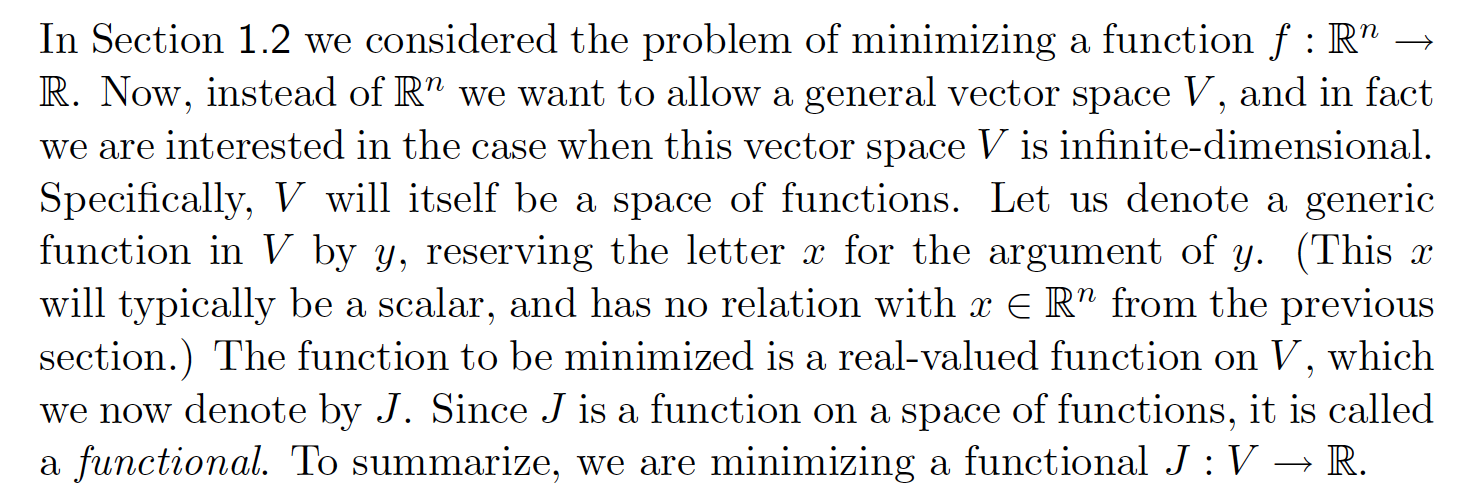
\includegraphics[width=\linewidth]{ch1/fig1.png}
    \end{figure}
\end{frame}

\begin{frame}{Norms for function spaces}
    \begin{itemize}
        \item We will frequently work with the function space $V = \mathcal{C}^k([a,b], \mathbb{R}^n)$ whose elements are k-times differentiable.
        \item The two norms that we will be focusing on are
        \begin{itemize}
            \item 0-norm:
            \begin{equation}
                \Vert y \Vert_0 = \max_{a \leq x \leq b} \vert y(x) \vert
            \end{equation}
            $y \in V$ and $\vert \cdot \vert$ is just the euclidean norm.
            \item 1-norm:
            \begin{equation}
                \Vert y \Vert_1 = \max_{a \leq x \leq b} \vert y(x) \vert + \max_{a \leq x \leq b} \vert y'(x) \vert
            \end{equation}
            $y \in V$ and $\vert \cdot \vert$ is just the euclidean norm.
        \end{itemize}
    \end{itemize}
\end{frame}

\begin{frame}{Local minima of a functional}
    \begin{figure}
        \centering
        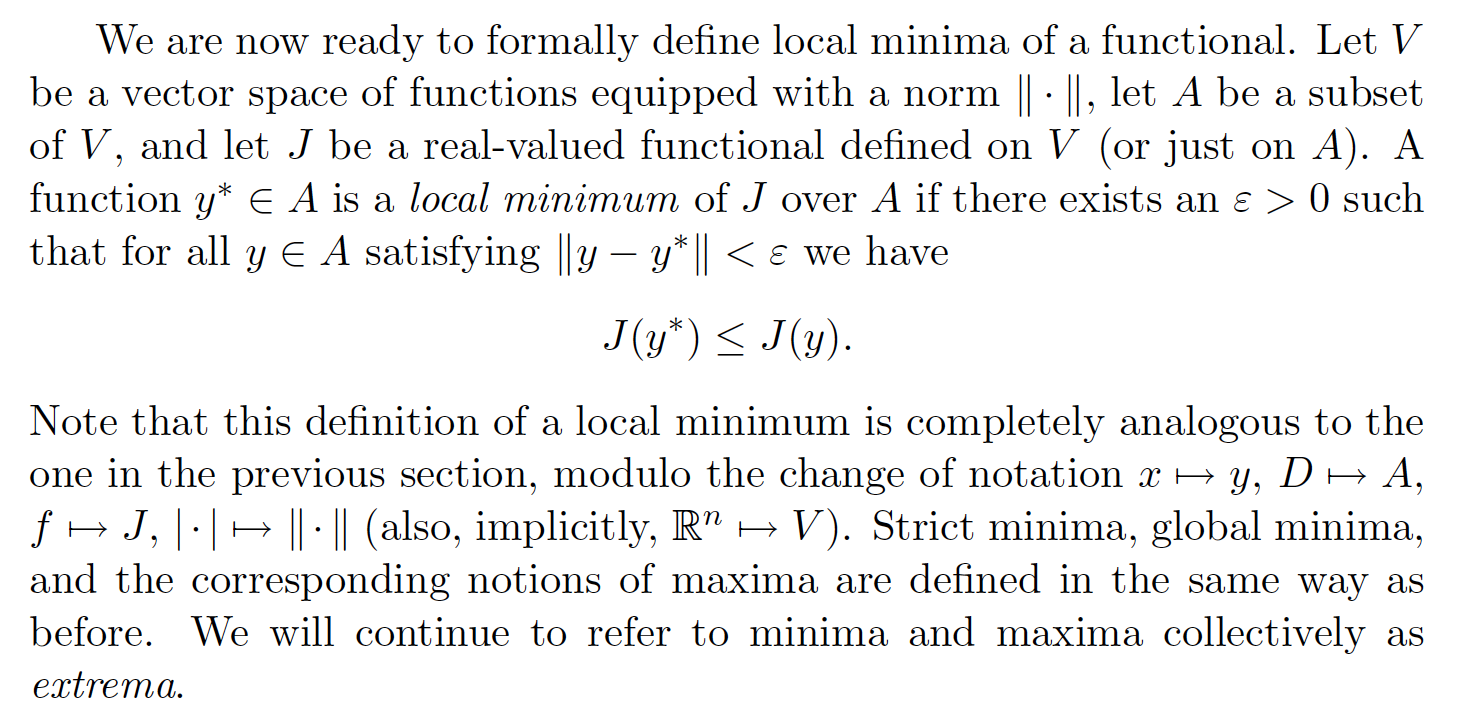
\includegraphics[width=\linewidth]{ch1/fig2.png}
    \end{figure}
\end{frame}

\begin{frame}{First variation}
     \begin{figure}
        \centering
        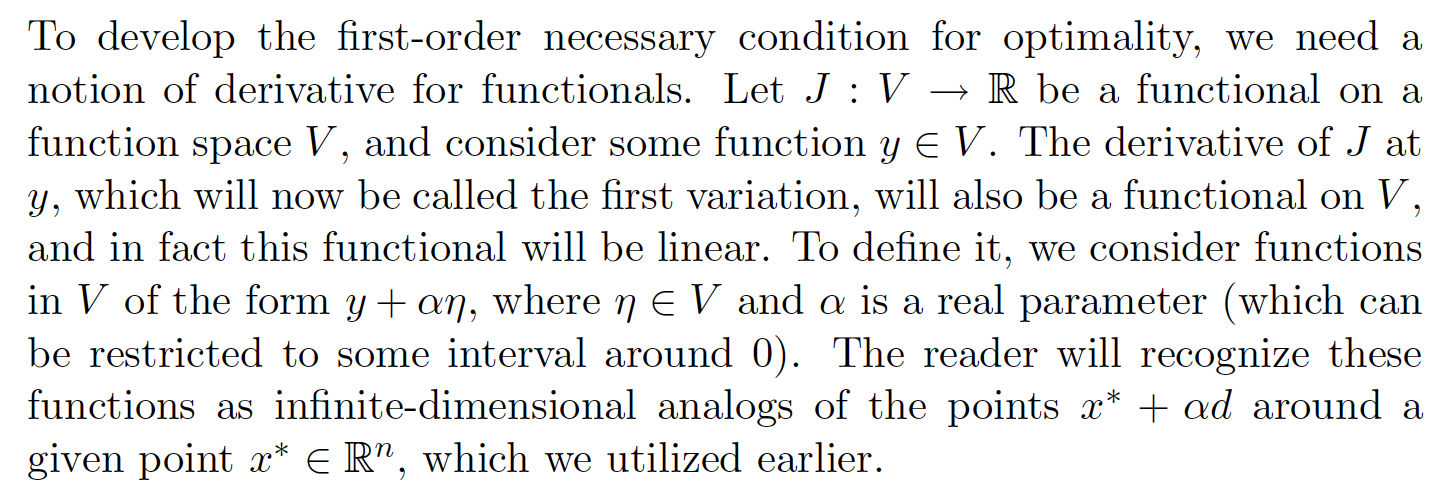
\includegraphics[width=\linewidth]{ch1/fig3.png}
    \end{figure}
\end{frame}

\begin{frame}{First variation}
    \begin{figure}
        \centering
        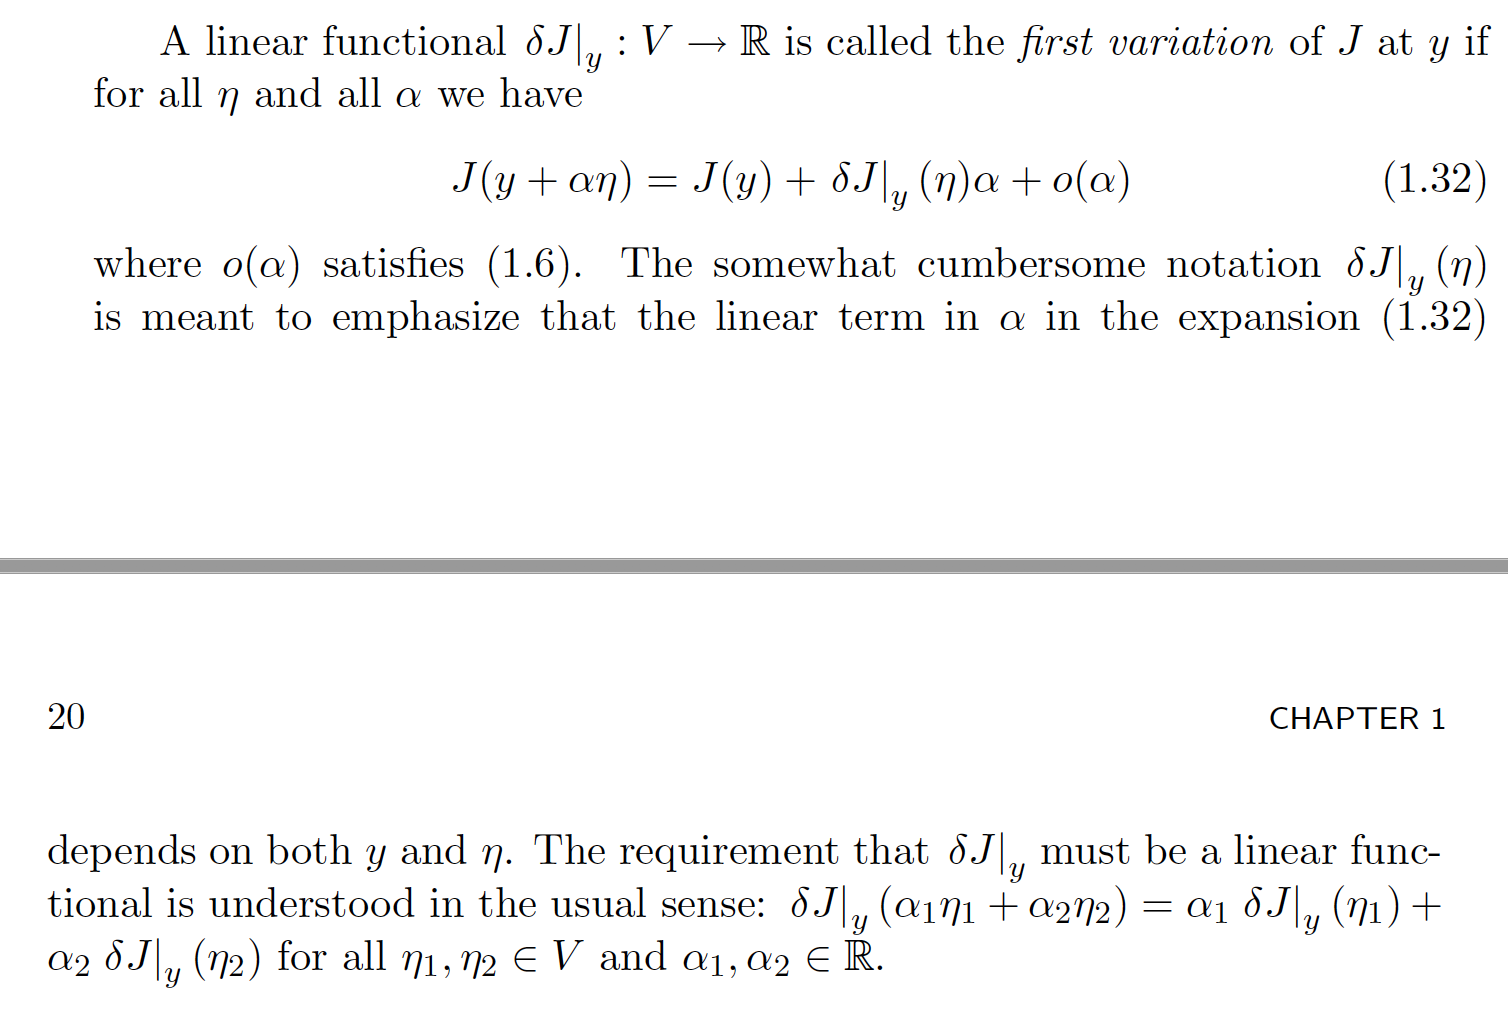
\includegraphics[width=\linewidth]{ch1/fig4.png}
    \end{figure}
\end{frame}

\begin{frame}{First variation}
    \begin{figure}
        \centering
        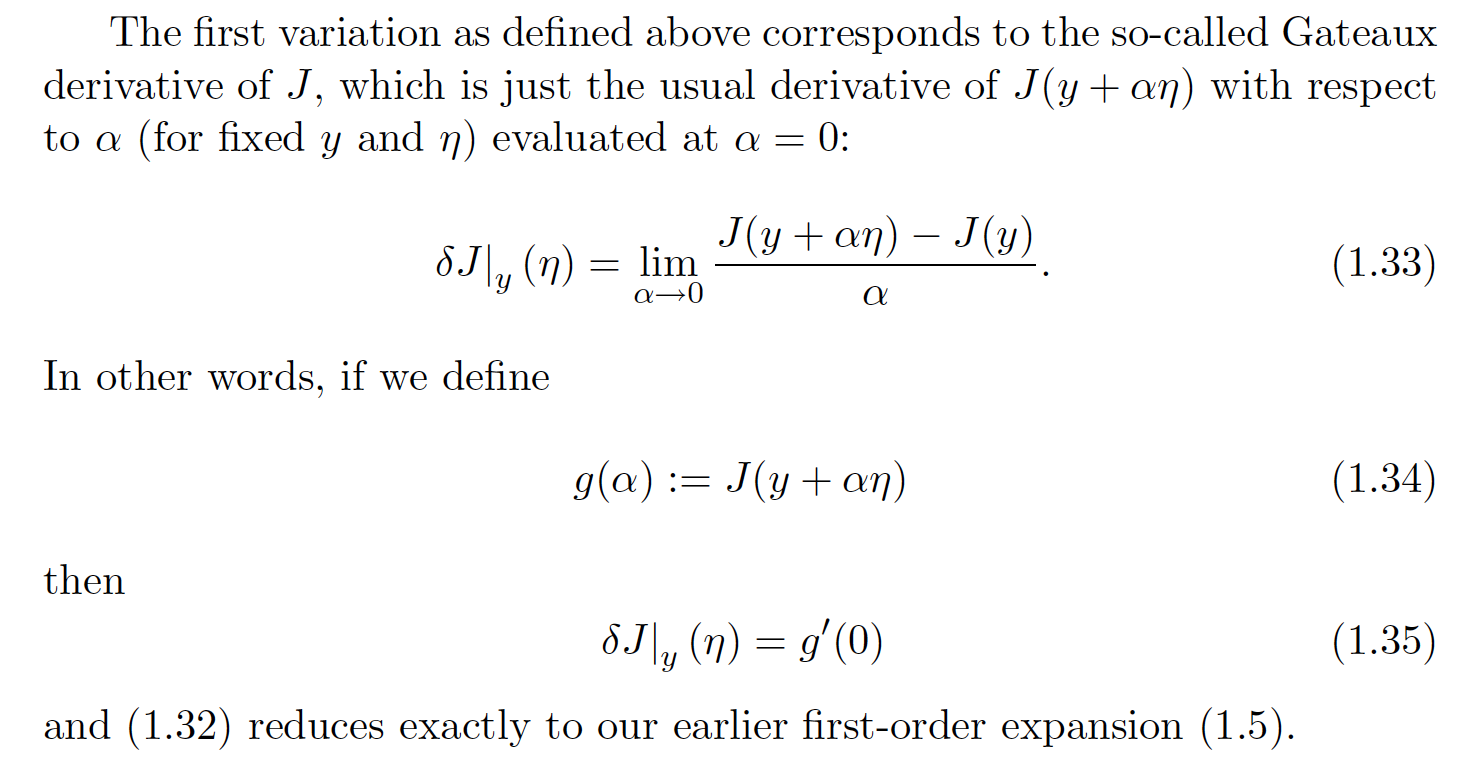
\includegraphics[width=\linewidth]{ch1/fig5.png}
    \end{figure}
\end{frame}


\begin{frame}{First-order necessary condition}
    \begin{itemize}
        \item Now, suppose that $y^*$ is a local min of J over some subset $A$ of $V$.
        \item $\eta \in V$ is a perturbation which will be commonly used throughout the book.
        \item $\eta$ is an admissible perturbation if $y + \alpha \eta \in A$ for $\alpha$ close to 0.
        \item By the same logic used in finite-dimensional optimization, we get to the \textbf{first-order necessary condition for optimality}: \textit{$\delta J \vert_{y^*} (\eta) = 0$ for all admissible perturbations, $\eta$}.
    \end{itemize}
\end{frame}

\begin{frame}{Basic calculus of variations problem}
\begin{itemize}
    \item Consider a function $L: \mathbb{R} \times \mathbb{R}^n \times \mathbb{R}^n \rightarrow \mathbb{R}$
    \item Among all $\mathcal{C}^1$ curves $y:[a, b] \rightarrow \mathbb{R}^n$ satisfying given boundary conditions
    \begin{equation}
        y(a) = y_0, \quad y(b) = y_1
    \end{equation}
    find the (local) minima of the cost functional
    \begin{equation}
        J(y) = \int_a^b L(x, y(x), y'(x))dx
    \end{equation}
    \item L is called the \textit{Lagrangian} or \textit{running cost}.
    \item Important: Even though $y$ and $y'$ are dependent, L is to be viewed as a function of three independent variables!
\end{itemize}
\end{frame}

\begin{frame}{Weak and Strong Extrema}
    \begin{figure}
        \centering
        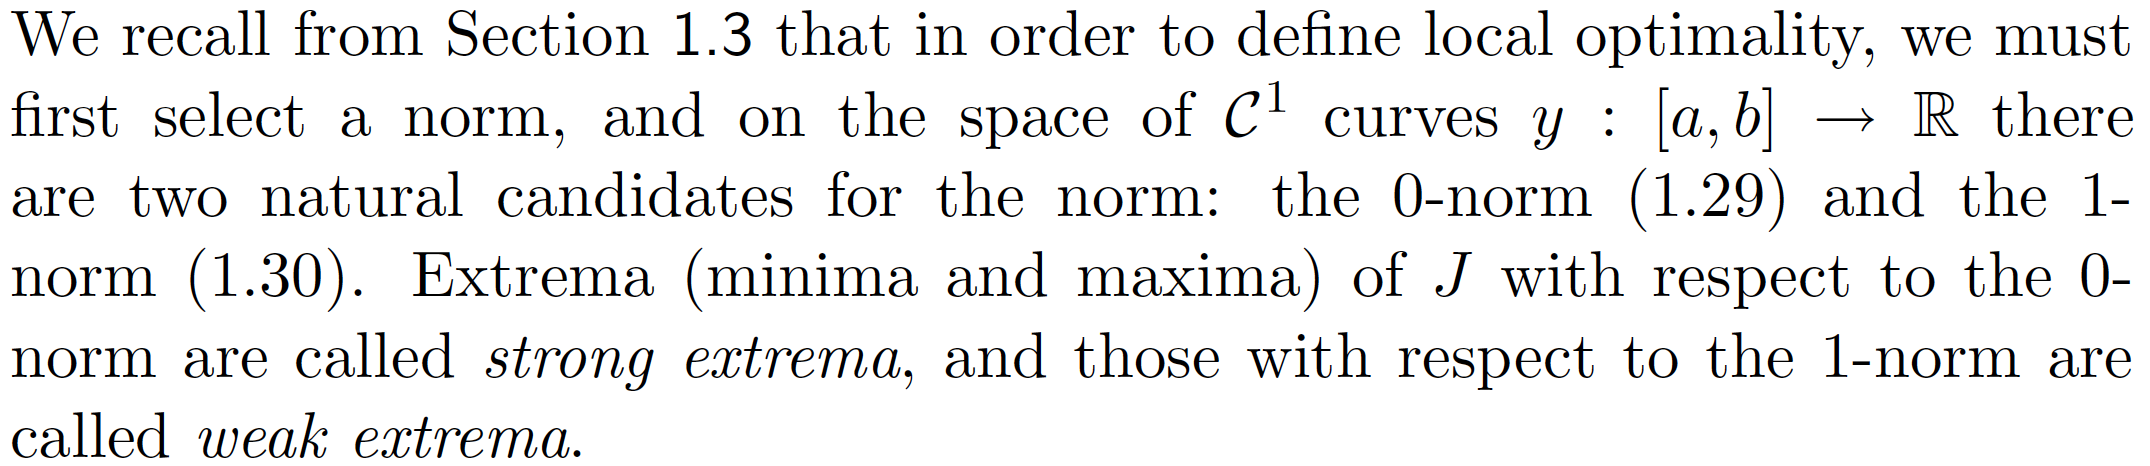
\includegraphics[width=\linewidth]{ch2/fig7.png}
    \end{figure}

    \begin{figure}
        \centering
        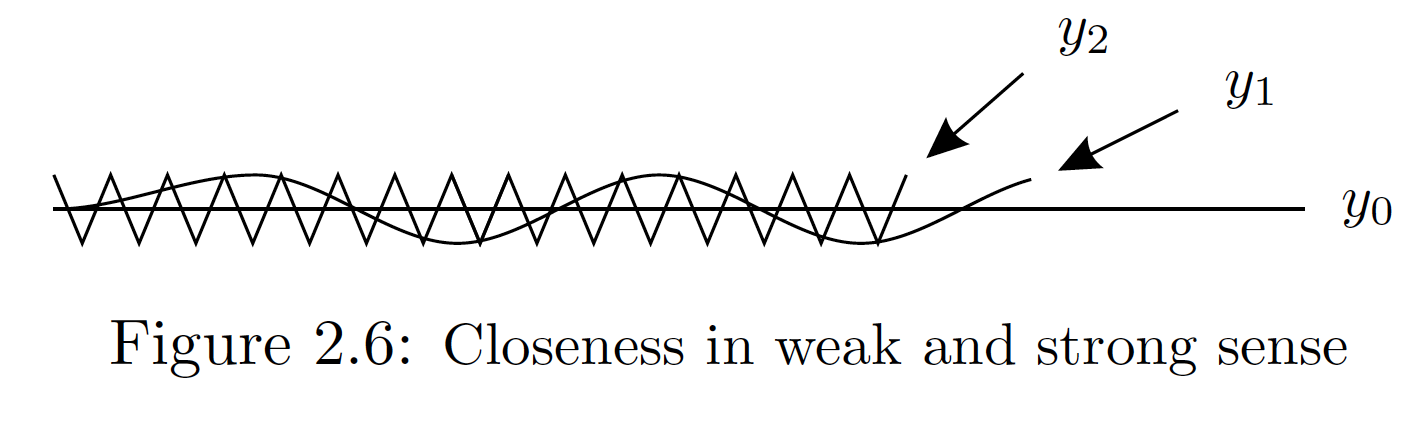
\includegraphics[width=\linewidth]{ch2/fig8.png}
    \end{figure}
\end{frame}

\begin{frame}{First-order necessary conditions for weak extrema}
    \begin{figure}
        \centering
        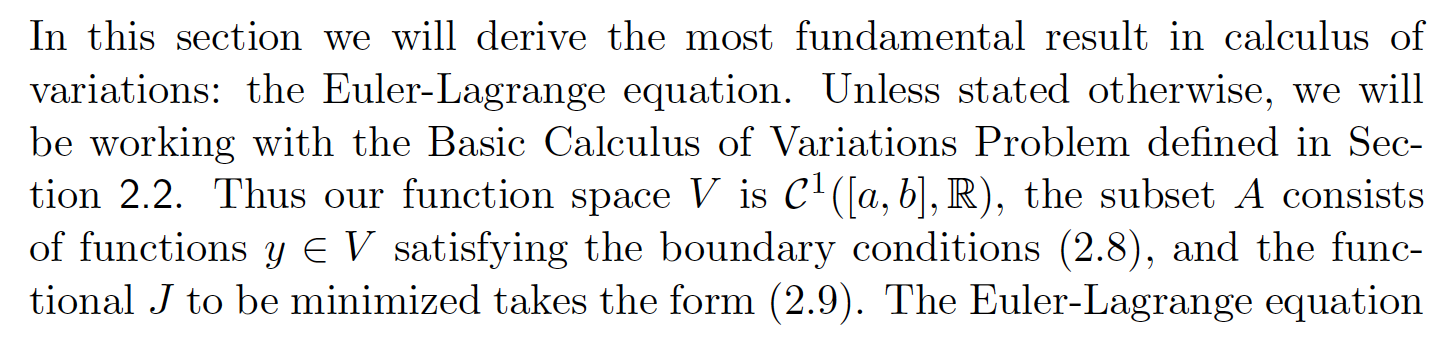
\includegraphics[width=\linewidth]{ch2/fig9.png}
    \end{figure}
    Notation: $L_x, L_y, L_z, L_{xx}, L_{xy},$ etc. are the partial derivatives of the Lagrangian $L = L(x, y, z)$.
\end{frame}

\begin{frame}{Euler-Lagrange equation}
    \begin{figure}
        \centering
        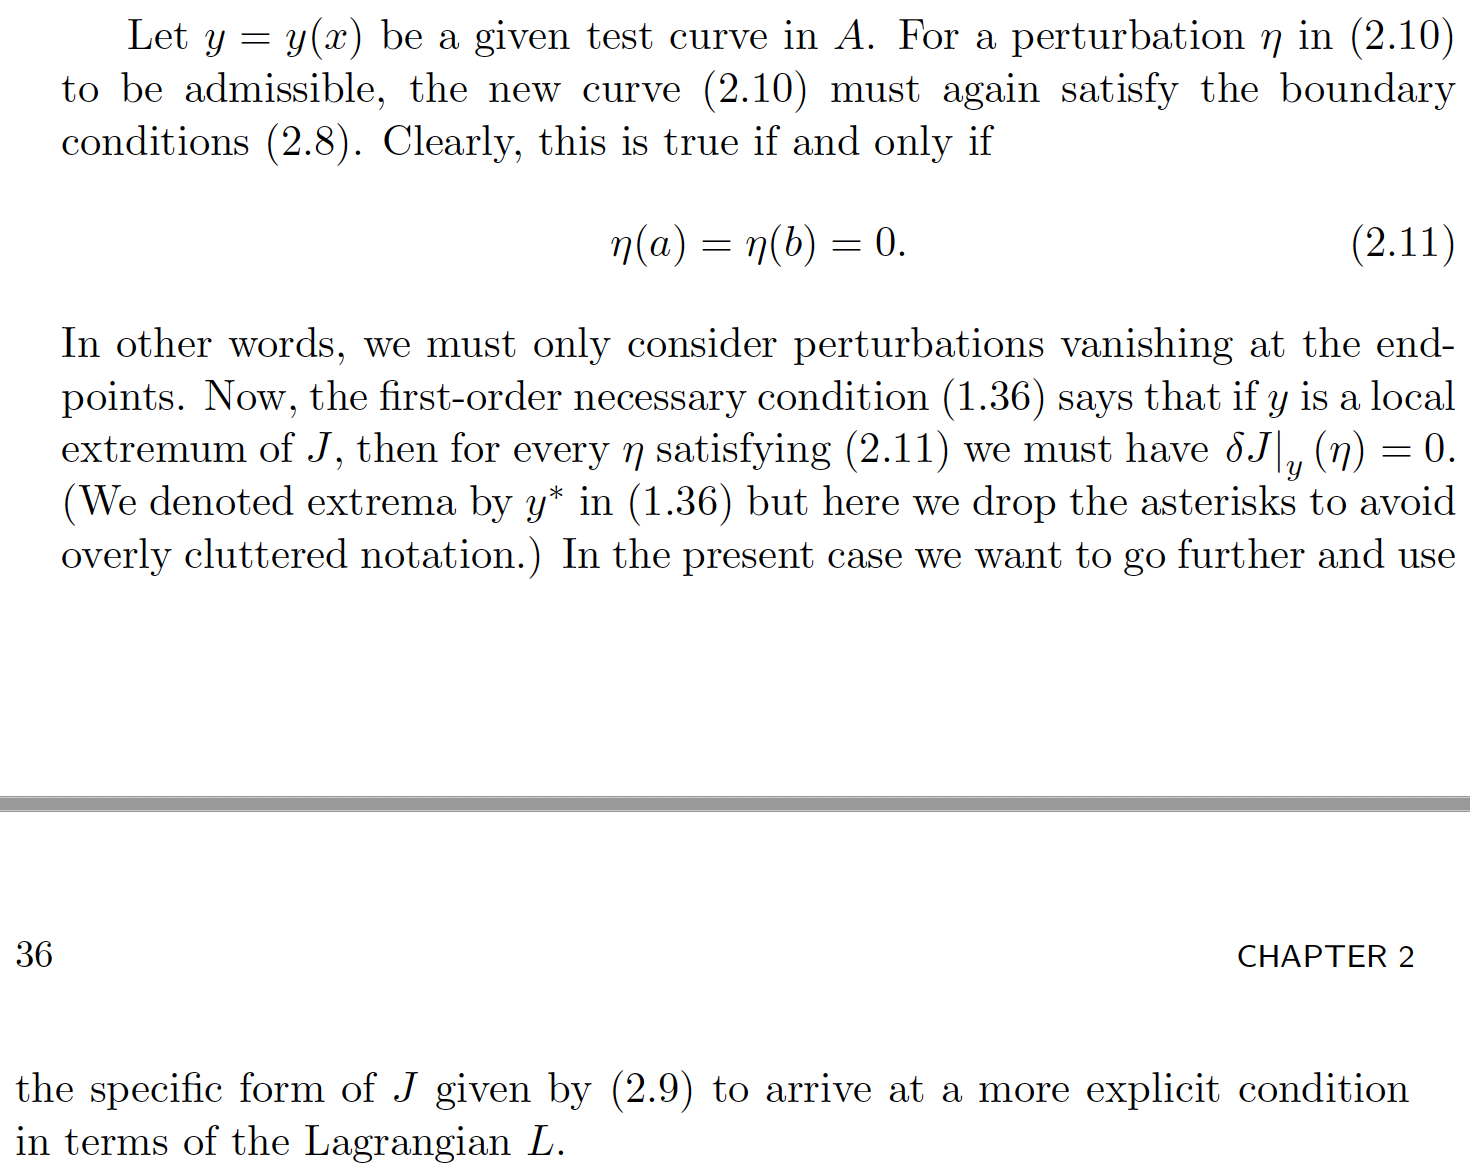
\includegraphics[width=0.9\linewidth]{ch2/fig10.png}
    \end{figure}
\end{frame}

\begin{frame}{Euler-Lagrange equation}
    \begin{itemize}
        \item The first variation, $\delta J\vert_y$ was defined via
        \begin{equation}
            J(y + \alpha \eta) = J(y) + \delta J\vert_y(\eta) \alpha + o(\alpha)
        \end{equation}
        We want to leverage the specific form of $J$ to get an explicit expression for $\delta J\vert_y$.
        \item We know that
        \begin{equation}
            J(y + \alpha \eta) = \int_a^b L(x, y(x) + \alpha \eta(x), y'(x) + \alpha \eta'(x))dx
        \end{equation}
        \item We can get the first order Taylor series of $J(y + \alpha \eta)$ wrt $\alpha$ around $\alpha=0$ by first taking the first order Taylor series of $L$ and then integrating it!
    \end{itemize}
\end{frame}

\begin{frame}{Euler-Lagrange equation}
    \begin{itemize}
        \item The first-order Taylor series of $L$ is
        \begin{align*}
            L(x, y + \alpha \eta, y' + \alpha \eta') &= L(x, y, y') +\\
            & \alpha (L_y(x, y, y')\eta + L_z(x, y, y')\eta') + o(\alpha)
        \end{align*}
        \item Integrating the above, we see that the first-order Taylor series of $J$ is
        \begin{align*}
            J(x, y + \alpha \eta, y' + \alpha \eta') &= \int_a^b [L(x, y, y') +\\
            & \alpha (L_y(x, y, y')\eta + L_z(x, y, y')\eta') + o(\alpha)]dx
        \end{align*}
        \item Comparing the first-order Taylor series of $J$ and the definintion of first variation, we arrive at an explicit expression for $\delta J\vert_y$
        \begin{equation*}
            \delta J\vert_y (\eta) = \int_a^b [L_y(x, y, y')\eta + L_z(x, y, y')\eta']dx
        \end{equation*}
    \end{itemize}
\end{frame}

\begin{frame}{Euler-Lagrange equation}
\begin{itemize}
    \item $\delta J \vert_y$ depends on both $\eta$ and $\eta'$. We can remove the dependence of $\eta'$ by using integration by parts
    \begin{align*}
        \delta J\vert_y (\eta) &= \int_a^b L_y(x, y, y')\eta dx + \int_a^b L_z(x, y, y')\eta'dx \\
        &= \int_a^b L_y(x, y, y')\eta dx + \eta L_z(x, y, y')\vert_a^b \\
        &- \int_a^b \eta \frac{d}{dx}L_z(x, y, y')dx \\
        &= \int_a^b \eta[L_y(x, y, y') - \frac{d}{dx}L_z(x, y, y')] dx
    \end{align*}
\end{itemize}
\end{frame}

\begin{frame}{Euler-Lagrange equation}
\begin{itemize}
    \item We know that if $y$ is a local extremum then $\delta J\vert_y=0$ for all admissible $\eta$.
    \item This is true iff
    \begin{equation*}
        L_y(x, y, y') = \frac{d}{dx}L_z(x, y, y')   \quad (2.18)
    \end{equation*}
    where
    \begin{equation*}
        \frac{d}{dx}L_z(x, y, y') = L_{zx}(x, y, y') + L_{zy}(x, y, y')y' + L_{zz}(x, y, y')y'' \,\, (2.19)
    \end{equation*}
    \item This is the celebrated Euler-Lagrange equation providing the first-order necessary condition for optimality!
\end{itemize}
\end{frame}

\begin{frame}{Euler-Lagrange equation}
    \begin{figure}
        \centering
        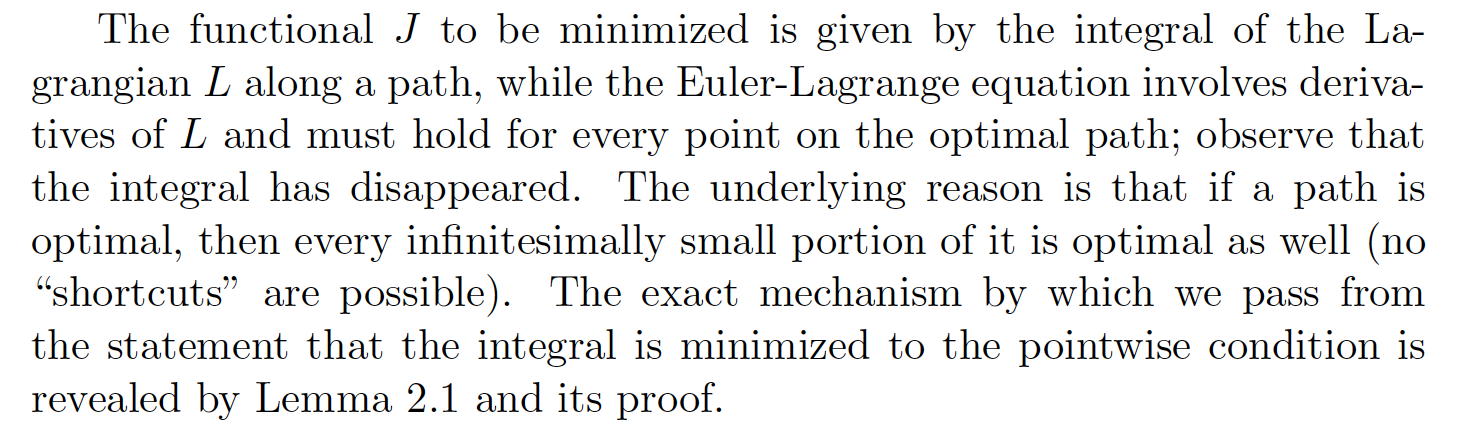
\includegraphics[width=\linewidth]{ch2/fig11.png}
    \end{figure}

    \begin{figure}
        \centering
        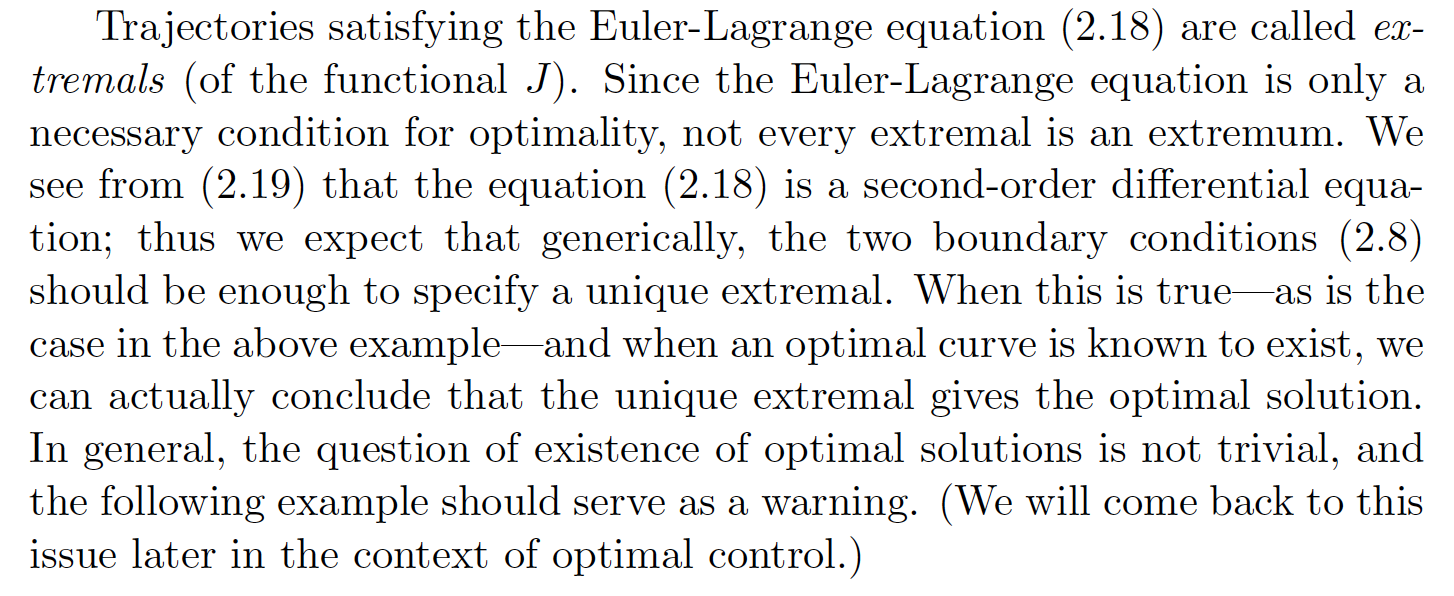
\includegraphics[width=\linewidth]{ch2/fig12.png}
    \end{figure}
\end{frame}

\begin{frame}{Euler-Lagrange for multiple dimensions}
    \begin{figure}
        \centering
        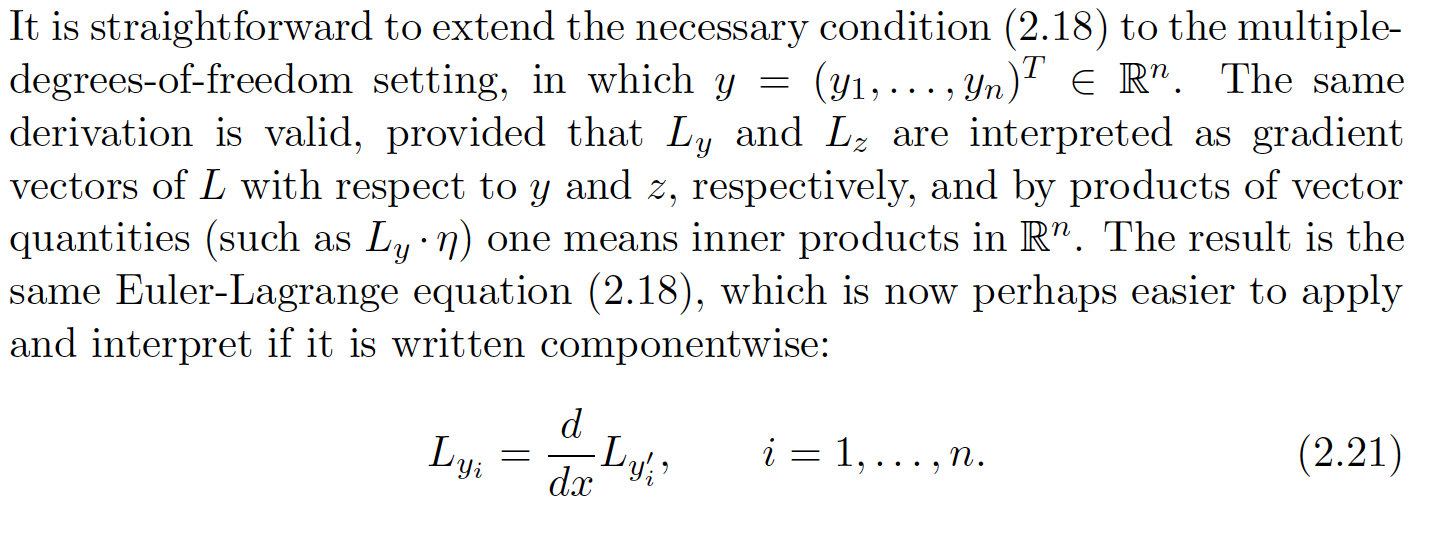
\includegraphics[width=\linewidth]{ch2/fig13.png}
    \end{figure}
\end{frame}

\begin{frame}{Special cases of Euler-Lagrange}
    \begin{figure}
        \centering
        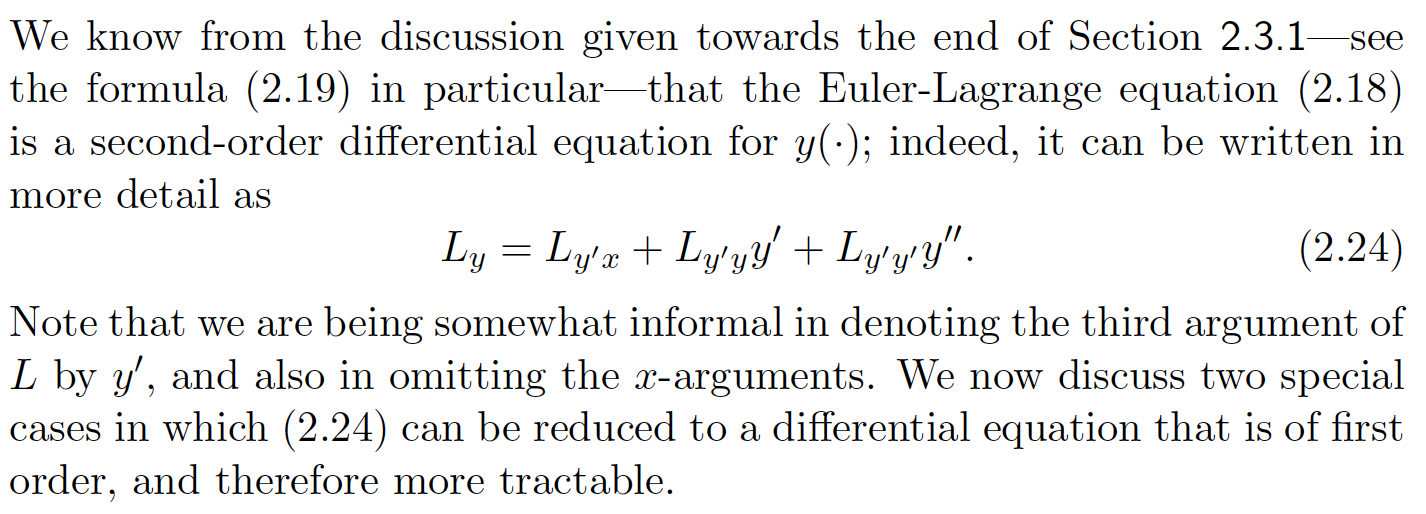
\includegraphics[width=\linewidth]{ch2/fig14.png}
    \end{figure}
\end{frame}

\begin{frame}{Special case 1 (no y)}
    \begin{figure}
        \centering
        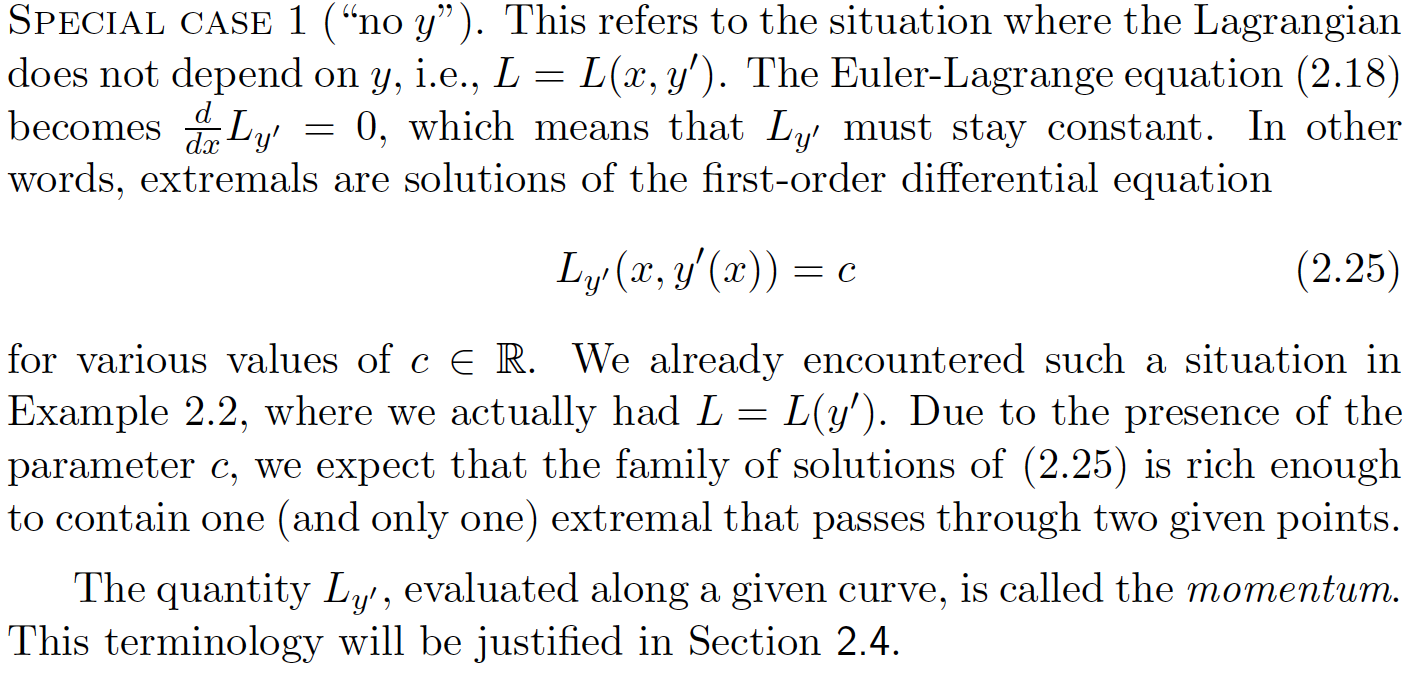
\includegraphics[width=\linewidth]{ch2/fig15.png}
    \end{figure}
\end{frame}

\begin{frame}{Special case 2 (no x)}
    \begin{figure}
        \centering
        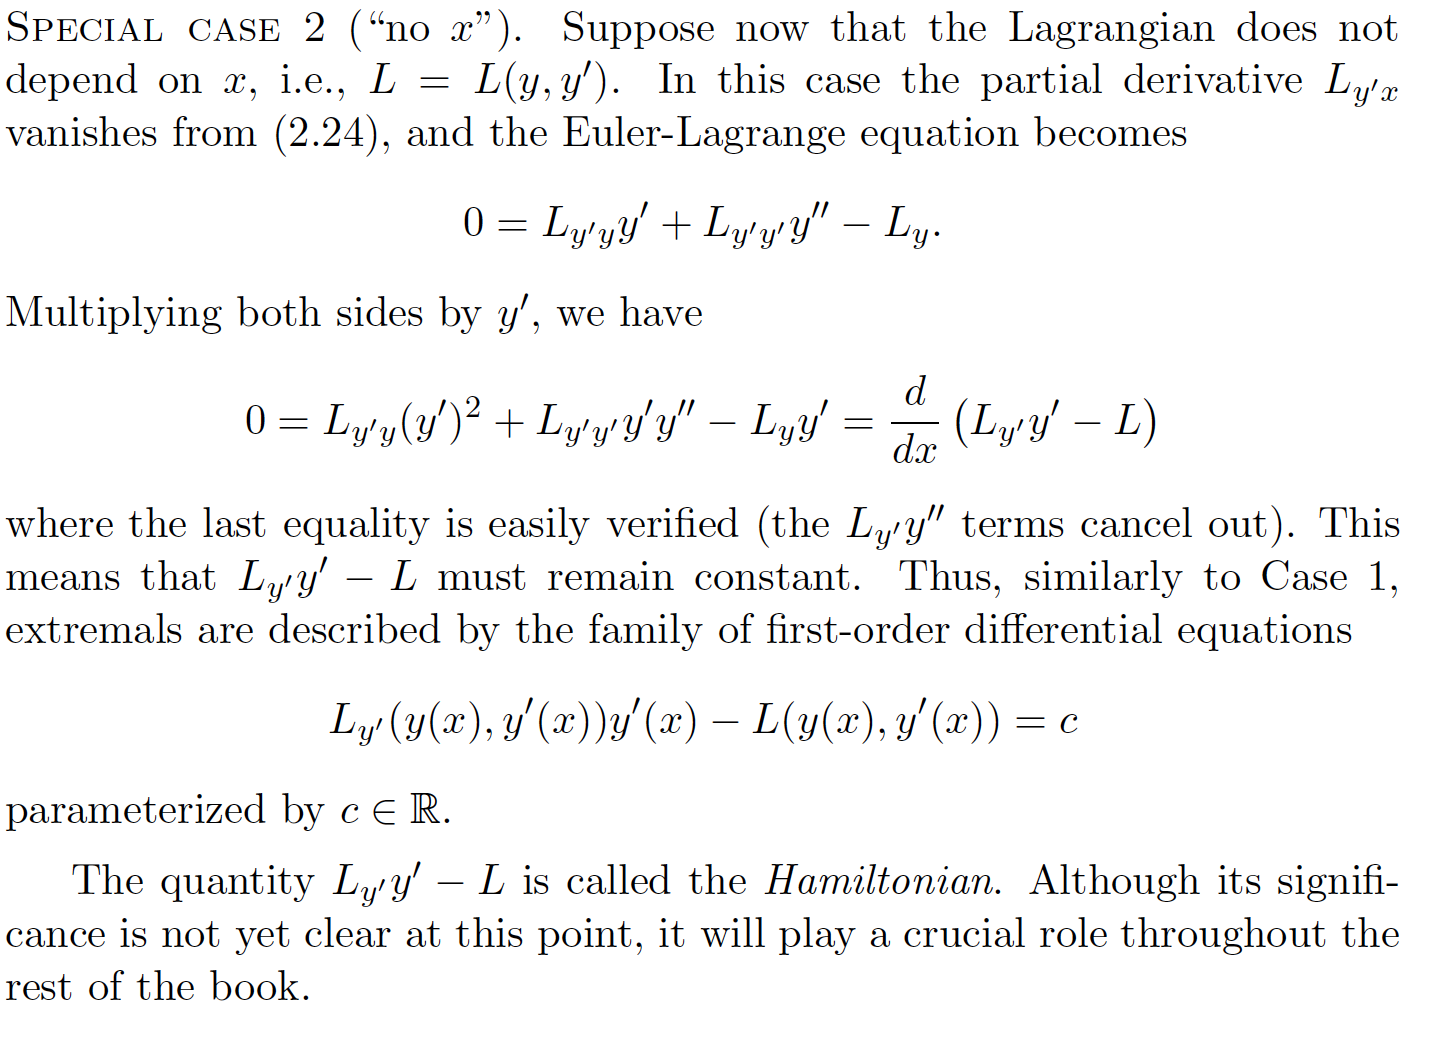
\includegraphics[width=\linewidth]{ch2/fig16.png}
    \end{figure}
\end{frame}

\begin{frame}{Variable-endpoint problem}
    \begin{figure}
        \centering
        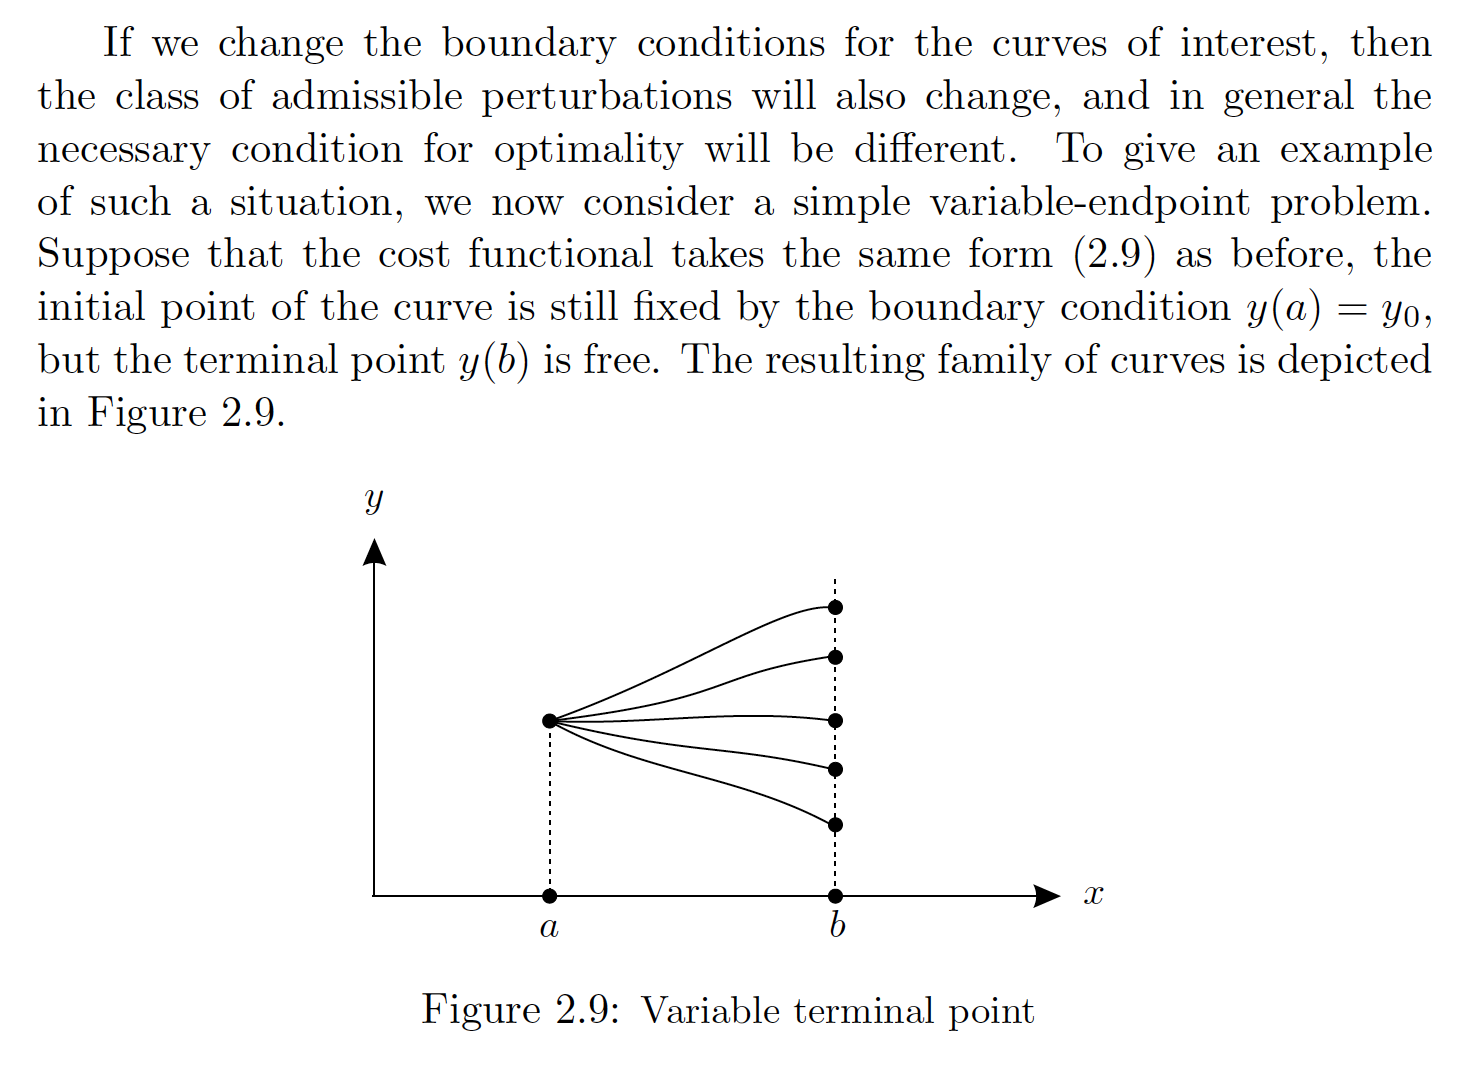
\includegraphics[width=\linewidth]{ch2/fig17.png}
    \end{figure}
\end{frame}

\begin{frame}{Variable-endpoint problem}
    \begin{figure}
        \centering
        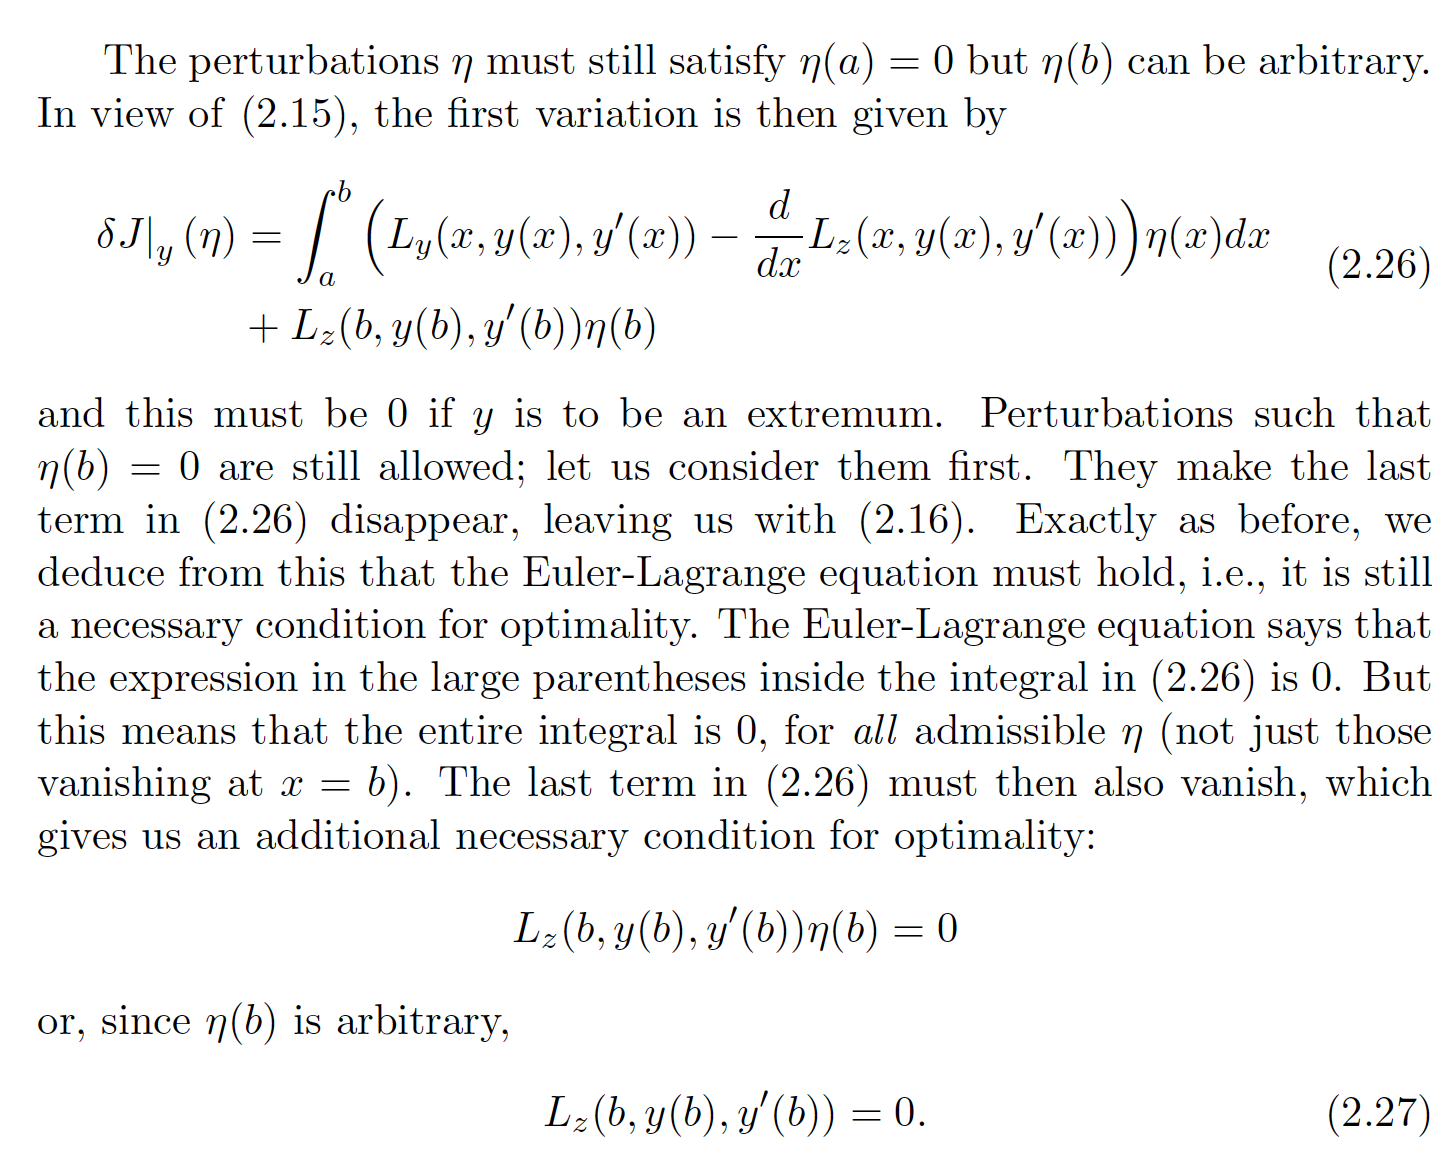
\includegraphics[width=\linewidth]{ch2/fig18.png}
    \end{figure}
\end{frame}


\begin{frame}{Hamilton's canonical equations}
    \begin{figure}
        \centering
        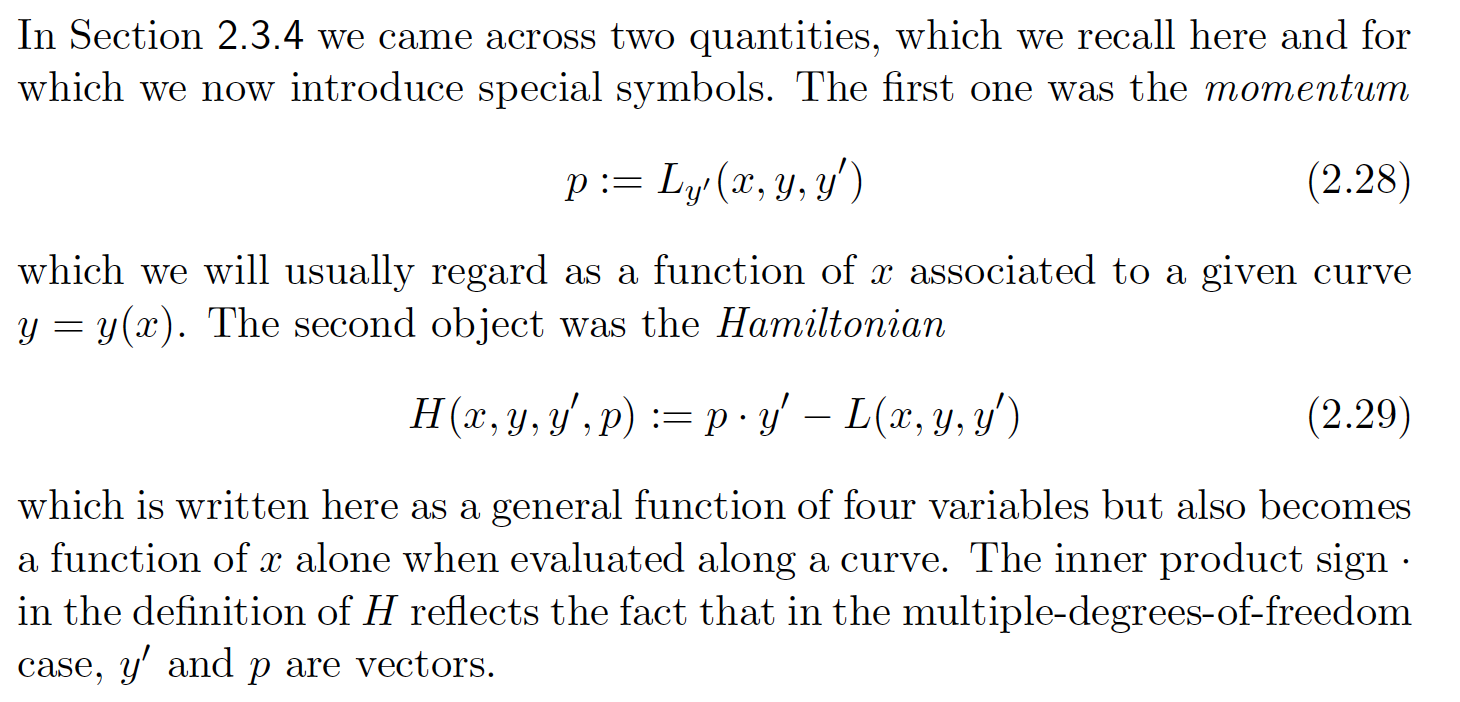
\includegraphics[width=\linewidth]{ch2/fig19.png}
    \end{figure}
\end{frame}

\begin{frame}{Hamilton's canonical equations}
    \begin{figure}
        \centering
        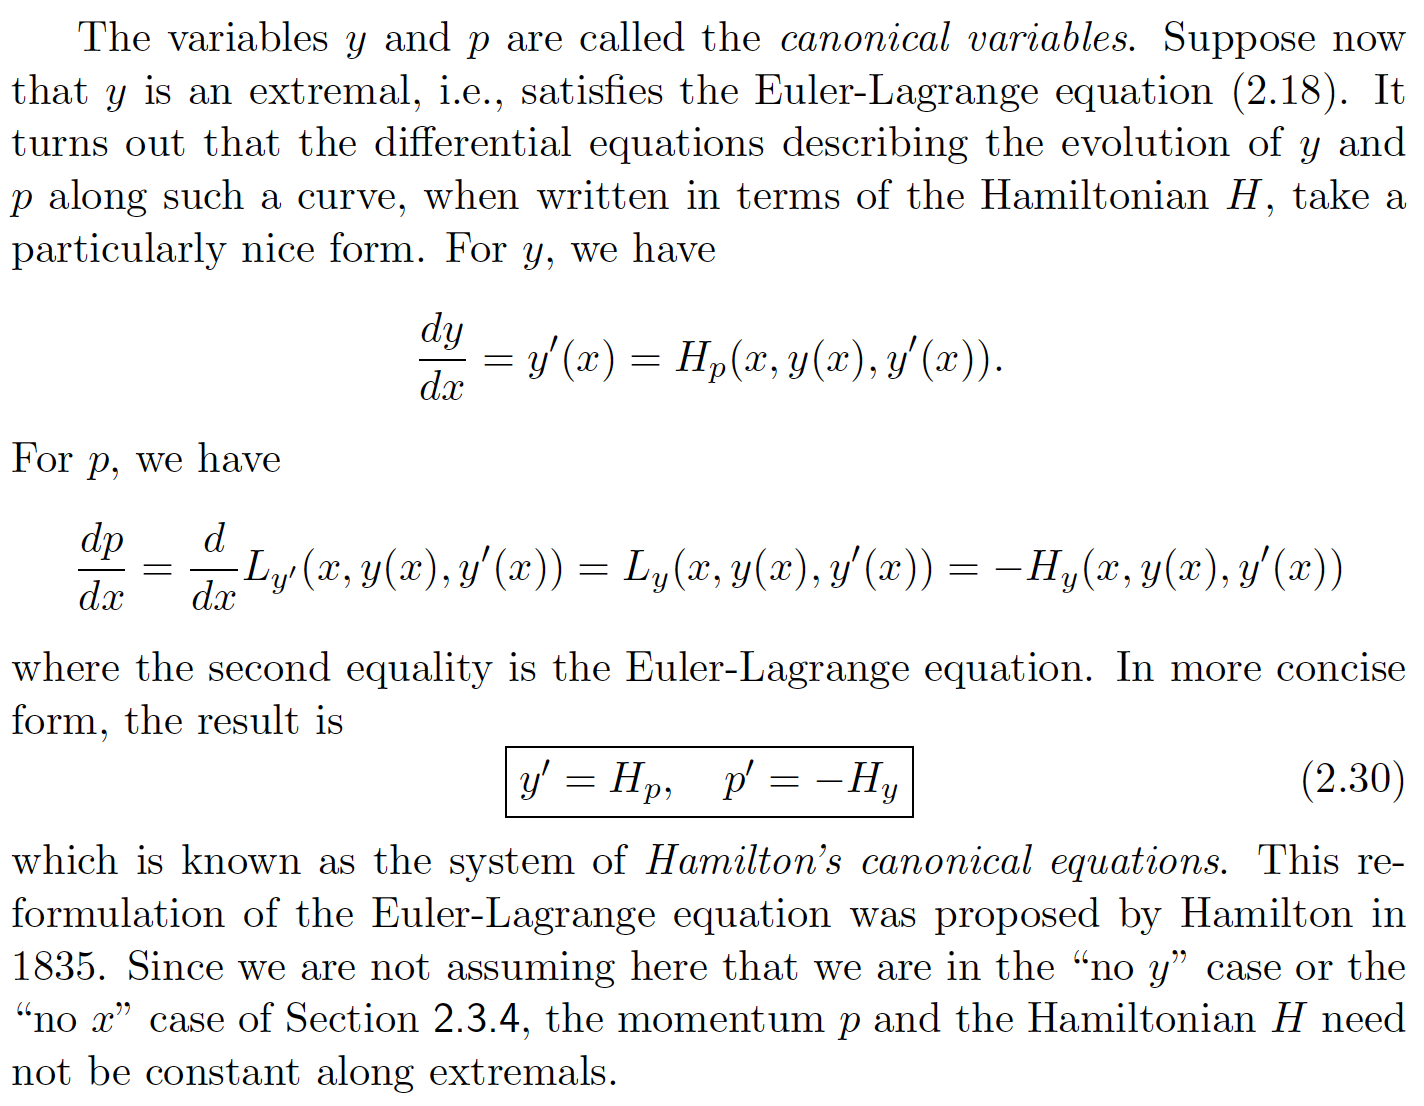
\includegraphics[width=0.9\linewidth]{ch2/fig20.png}
    \end{figure}
\end{frame}

\begin{frame}{Principle of least action}
    \begin{figure}
        \centering
        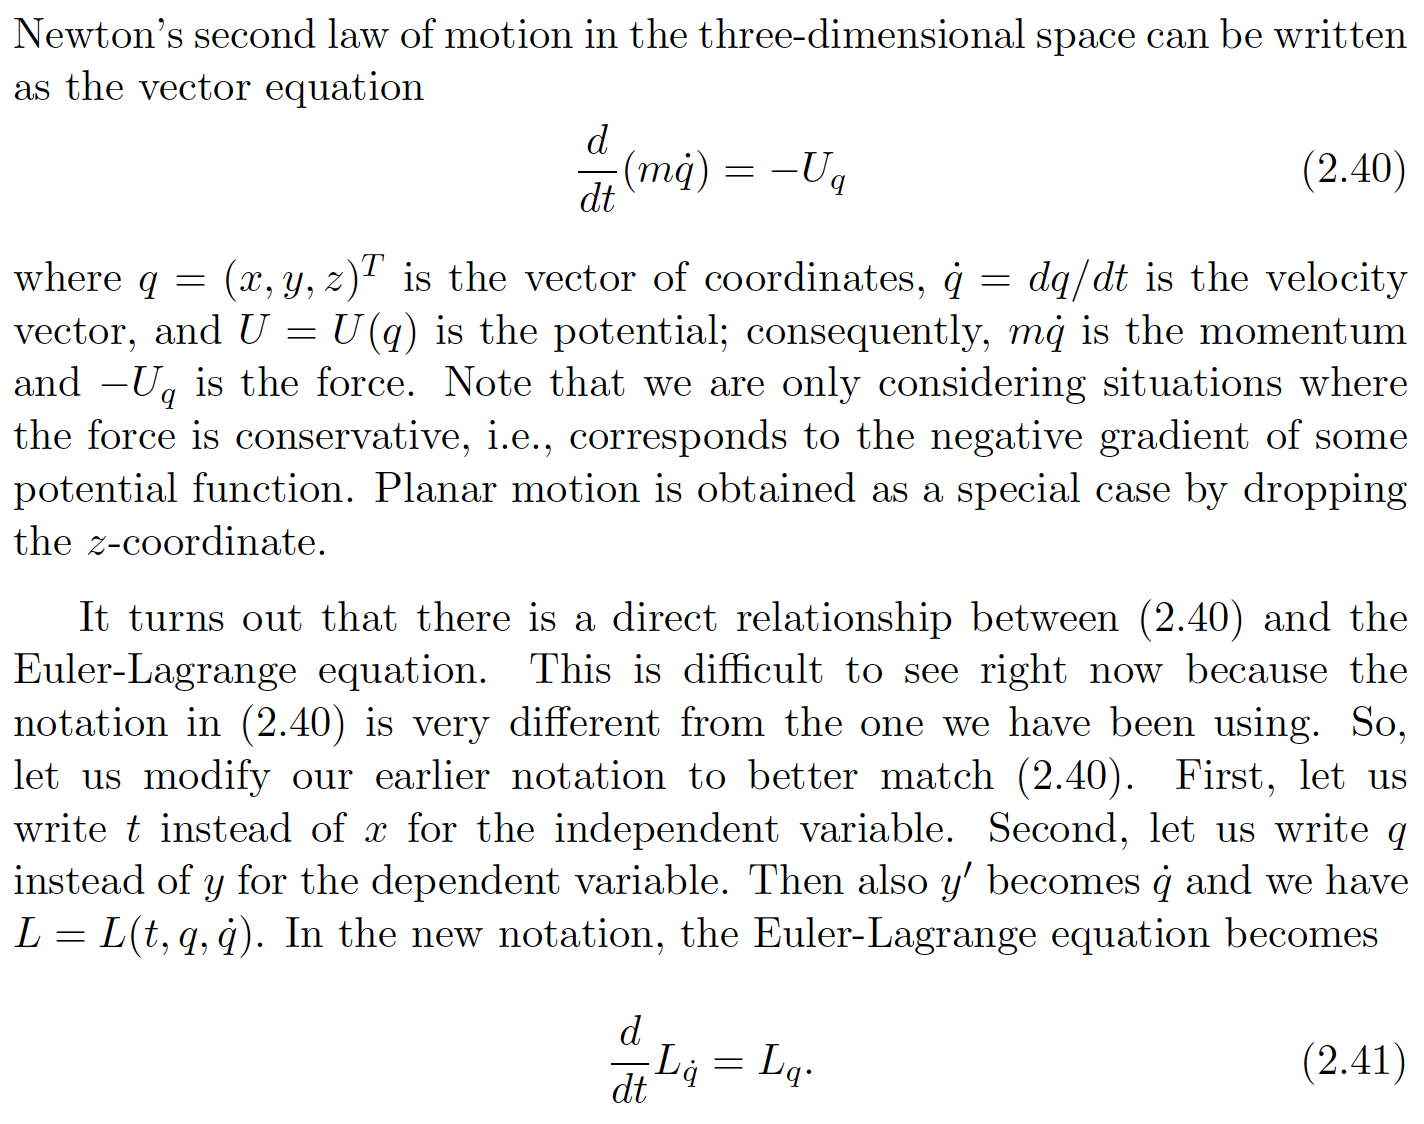
\includegraphics[width=0.9\linewidth]{ch2/fig21.png}
    \end{figure}
\end{frame}

\begin{frame}{Principle of least action}
    \begin{figure}
        \centering
        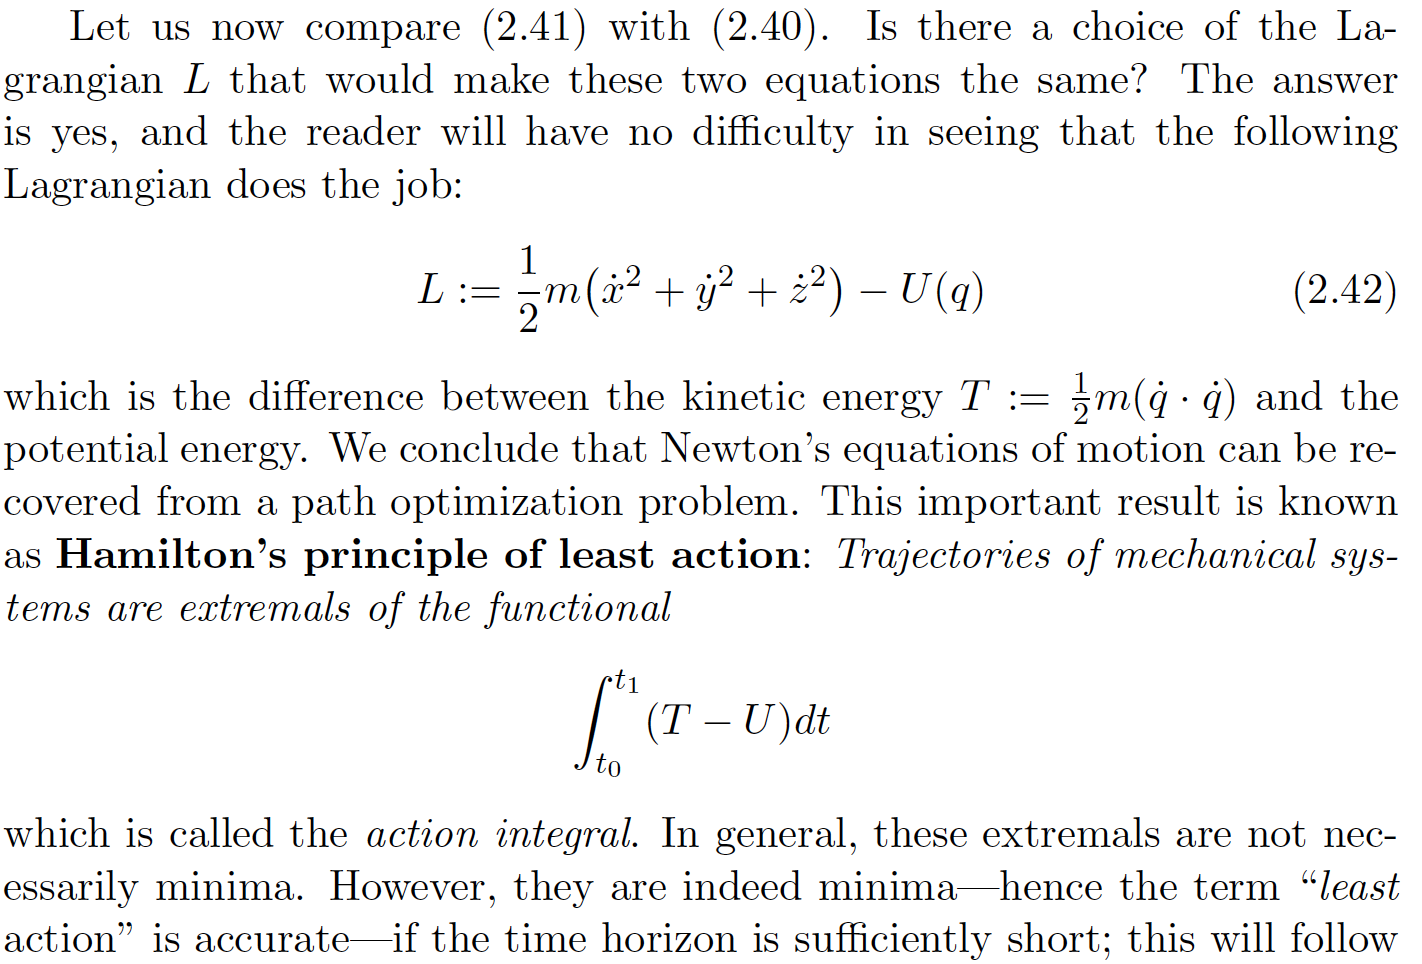
\includegraphics[width=0.9\linewidth]{ch2/fig22.png}
    \end{figure}
\end{frame}


\begin{frame}{Physical meaning of the Hamiltonian}
    \begin{figure}
        \centering
        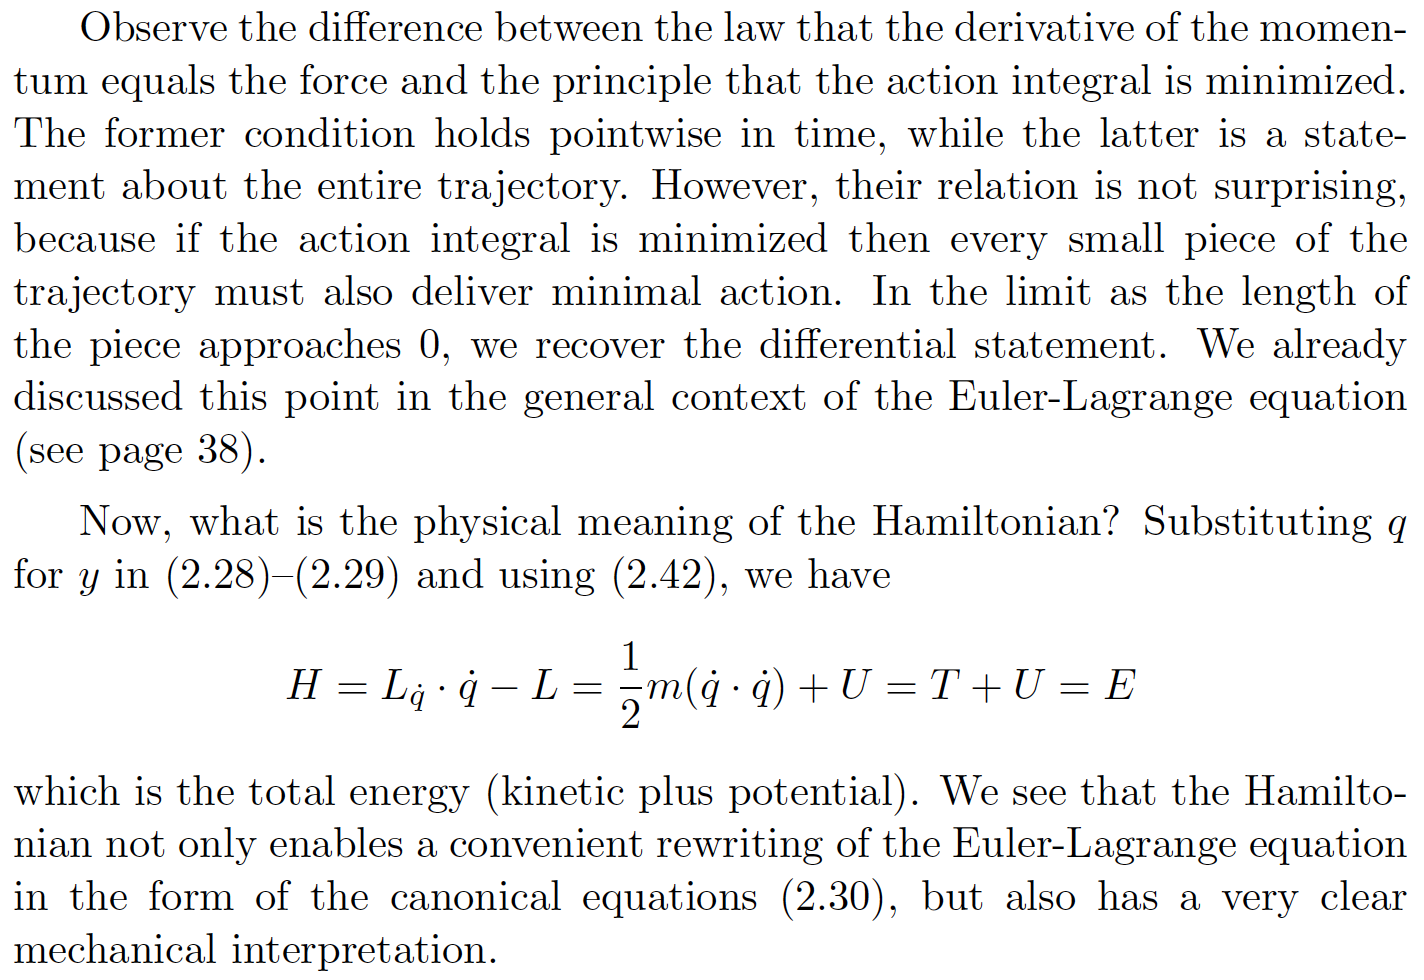
\includegraphics[width=0.9\linewidth]{ch2/fig23.png}
    \end{figure}
\end{frame}

\begin{frame}{Conservation of energy}
    \begin{figure}
        \centering
        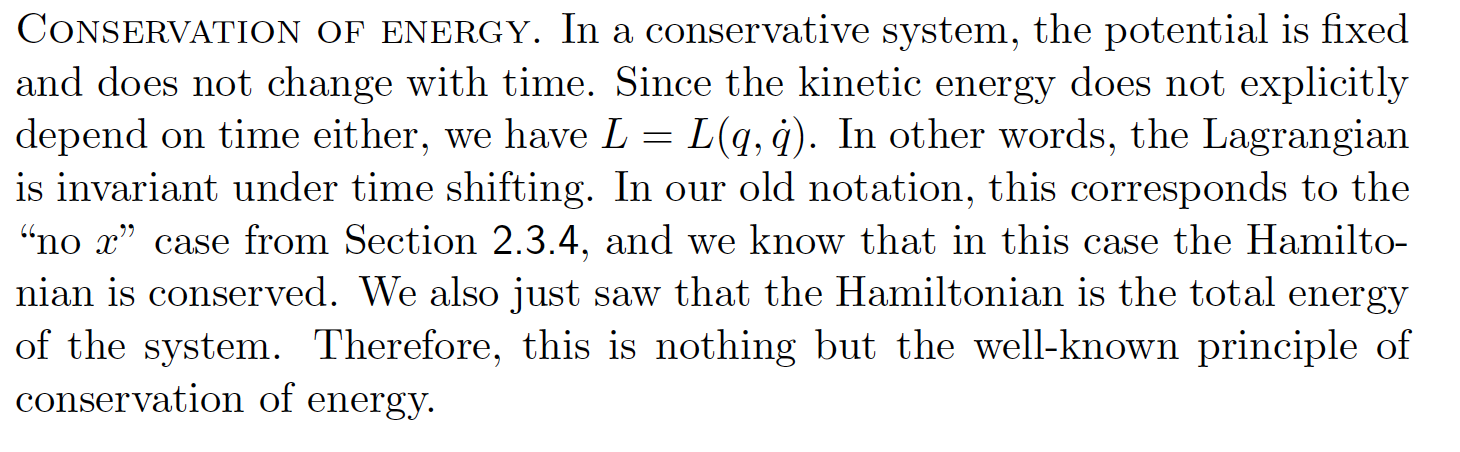
\includegraphics[width=\linewidth]{ch2/fig24.png}
    \end{figure}
\end{frame}

\begin{frame}{Conservation of momentum}
    \begin{figure}
        \centering
        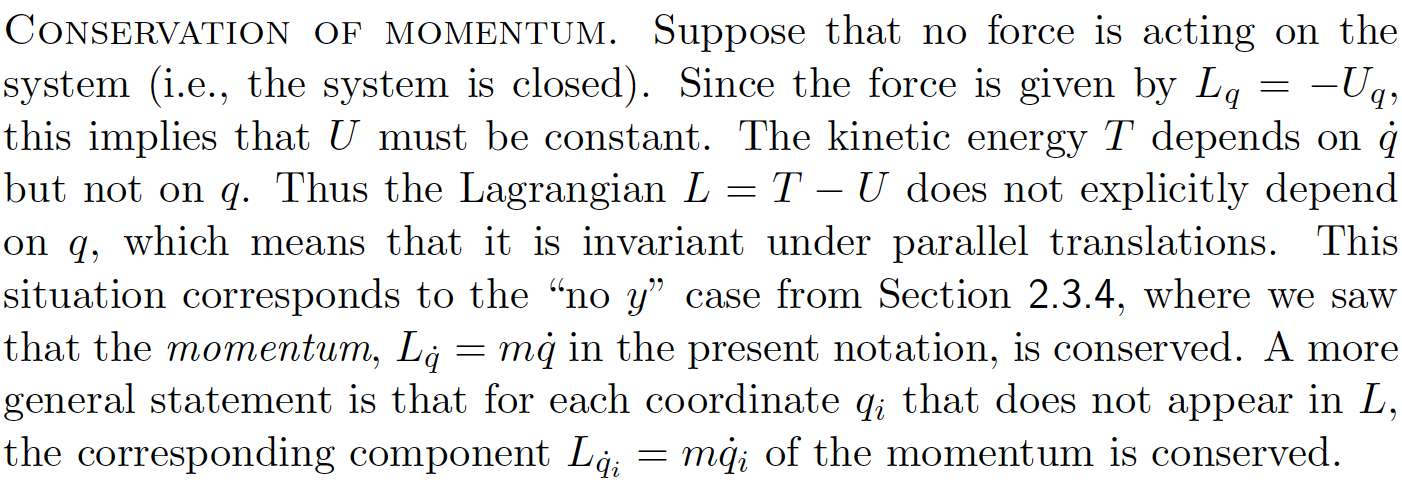
\includegraphics[width=\linewidth]{ch2/fig25.png}
    \end{figure}
\end{frame}

\begin{frame}{Integral Constraints}
    \begin{itemize}
        \item The basic calculus of variations problem is augmented with a constraint of the form
        \begin{equation}
            C(y) = \int_a^b M(x, y, y')dx = C_0.
        \end{equation}
        \item We once again work with the family of perturbed curves $y + \alpha \eta$ but now for $\eta$ to be admissible $y+\alpha \eta$ has to satisfy the boundary conditions and the constraint i.e. $C(y + \alpha \eta) = C_0$ for $\alpha$ close to 0.
        \item Satisfying the constraint implies that the first variation of $C$ is 0, $\delta C\vert_y(\eta) = 0.$
    \end{itemize}
\end{frame}

\begin{frame}{Integral Constraints}
    \begin{itemize}
        \item Using the same calculations that we did for deriving Euler-Lagrange we get that
        \begin{equation}
            \int_a^b[M_y(x, y, y') - \frac{d}{dx}M_z(x, y, y')]\eta dx = 0.
        \end{equation}
        \item So our basic first-order necessary condition is
        \begin{equation}
            \int_a^b(L_y - \frac{d}{dx}L_z)\eta dx = 0 \quad \forall \eta \,\, \textrm{s.t.} \int_a^b(M_y - \frac{d}{dx}M_z)\eta dx = 0
        \end{equation}
    \end{itemize}
\end{frame}

\begin{frame}{Integral Constraints}
    \begin{itemize}
         \item Similar to constrained finite-dimension optimization, we get that $\exists$ a constant $\lambda^*$ s.t.
         \begin{equation}
             (L_y - \frac{d}{dx}L_z) + \lambda^*(M_y - \frac{d}{dx}M_z)=0
         \end{equation}
         \item Rearranging terms we get
         \begin{equation}
             (L + \lambda^*M)_y = \frac{d}{dx}(L + \lambda^*M)_z
         \end{equation}
         which is the Euler-Lagrange equation for the augmented Lagrangian $L + \lambda^* M$.
    \end{itemize}
\end{frame}

\begin{frame}{Integral Constraints}
    \begin{figure}
        \centering
        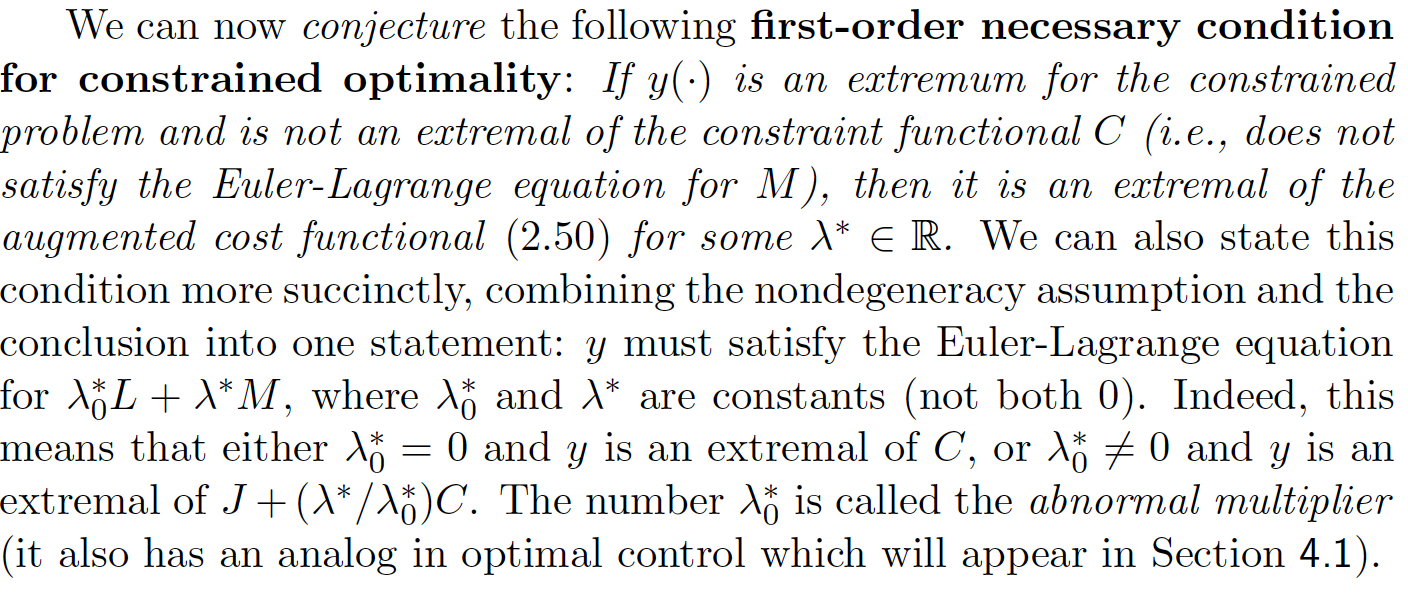
\includegraphics[width=\linewidth]{ch2/fig26.png}
    \end{figure}
\end{frame}

\begin{frame}{Non-integral Constraints}
    \begin{figure}
        \centering
        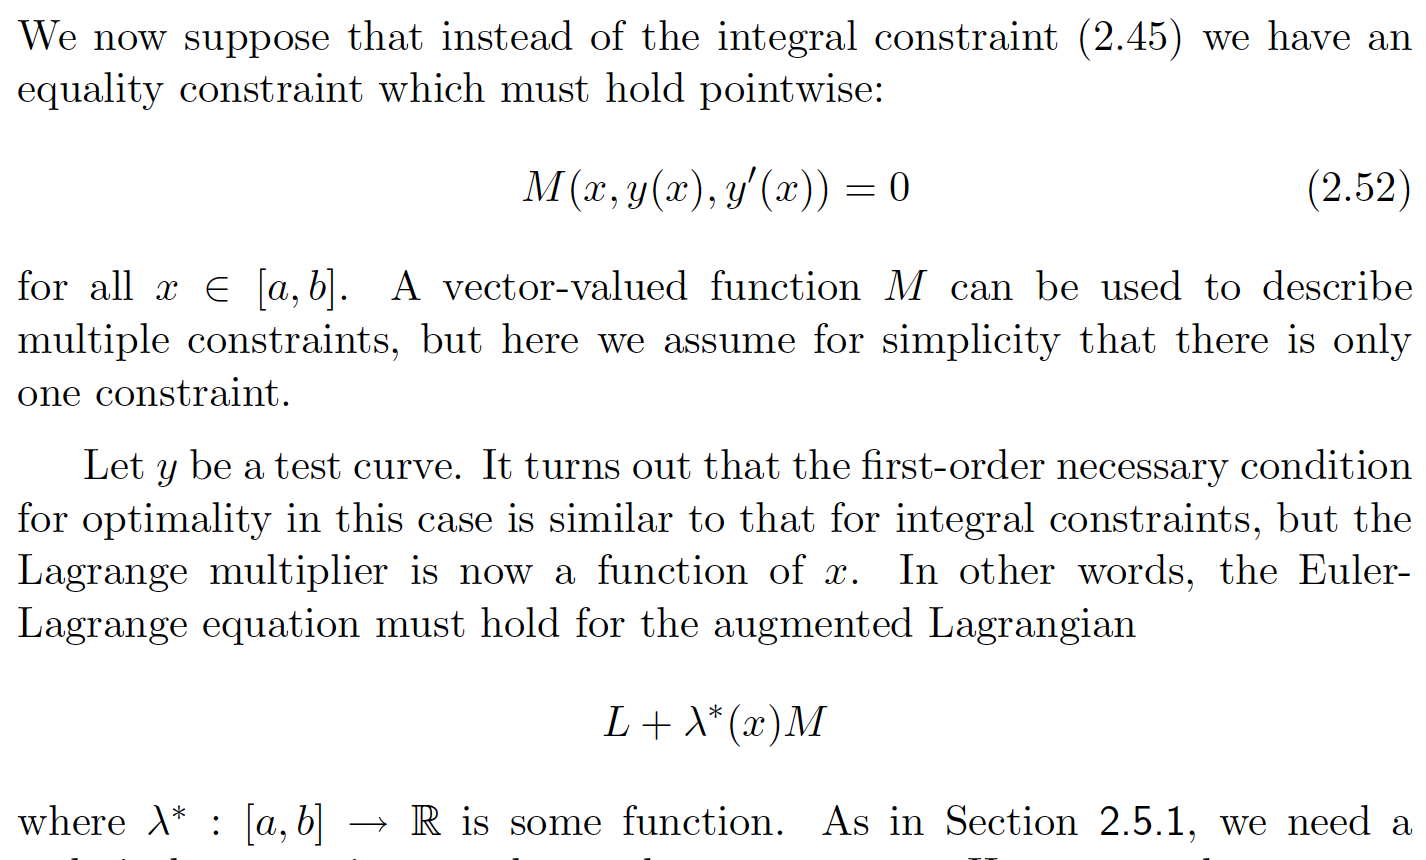
\includegraphics[width=\linewidth]{ch2/fig27.png}
    \end{figure}
\end{frame}

\begin{frame}{Loosening differentiability condtions}
    In calculus of variations we wanted to optimize a smooth functional with
    respect to a \(\mathcal{C}^1\) function. \\

    However, real life problems are often non-smooth e.g:
    \begin{itemize}
        \item Elastic collisions
        \item Refractions
        \item Catenary touching the ground
    \end{itemize}
    Much like in convex optimization we want to be able to deal with functions that are differentiable almost everywhere.
\end{frame}
    \begin{frame}
        \begin{figure}[!htb]
            \centering
            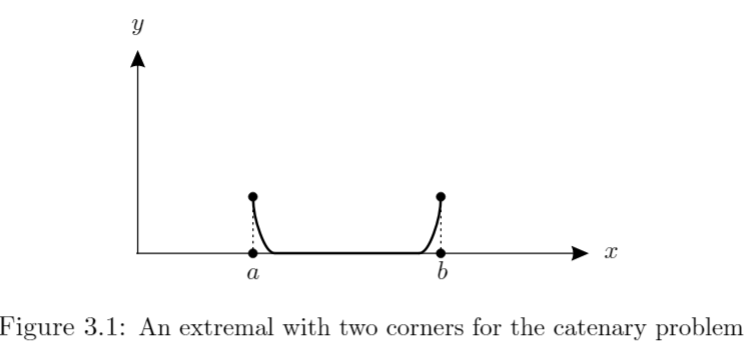
\includegraphics[width=0.95\textwidth]{img/Catenary.png}
            \caption{Liberzon p. 72}
            % \label{}
        \end{figure}
    \end{frame}
    \begin{frame}
        \begin{definition} [Piecewise \(\calC^1\) functions]
            A function $y$ is piecewise \(\calC^1\) on \(\left[a,b\right]\) if it's $\calC^1$
            everywhere except for a finite set of points where its derivative $y'$ is discontinuous.
        \end{definition}
        The points of discontinuity are called \emph{corner points}
        \begin{definition}[Corner point $c$]
            \(c \in \left[a,b\right]\) \\
            and \\
             \( y'(c^+) \defeq \lim_{x \searrow c} y'(x) \neq  y'(c^+) \defeq \lim_{x \nearrow c} y'(x)\)
        \end{definition}
    \end{frame}
    \begin{frame}
        \begin{example}
            Consider the problem of minimizing the functional
            \(J ( y ) = \int _ { - 1 } ^ { 1 } y ^ { 2 } ( x ) \left( y ^ { \prime } ( x ) - 1 \right)^ { 2 } d x
            \)\\
            s.t.
            \(y ( - 1 ) = 0 , \,  y ( 1 ) = 1 \)
        \end{example}

         It is clear that $J ( y ) \geq 0$ for all curves $y .$ We can find $\mathcal { C } ^ { 1 }$ curves giving $g$
        values of $J ( y )$ arbitrarily close to $0 ,$ but cannot achieve $J ( y ) = 0 .$ On the
        other hand, the curve
        \begin{equation*}
            y ( x ) = \left\{ \begin{array} { l l } { 0 } & { \text { if } - 1 \leq x < 0 } \\ { x } & { \text { if } 0 \leq x \leq 1 } \end{array} \right.
        \end{equation*}
        gives $J ( y ) = 0 .$ This curve is piecewise $\mathcal { C } ^ { 1 }$ with a corner point at $x = 0$
    \end{frame}
    \begin{frame}
        We need to generalize our notion of norms appropriately to handle functions with discontinuous derivatives the (\(\norm{\cdot}_0\) stays the same since it doesn't care about derivatives)
        \begin{definition}[Generalized 1-norm]\label{def:gen1norm}
            \begin{equation*}
                \| y \| _ { 1 } : = \max _ { a \leq x \leq b } | y ( x ) | + \max _ { a \leq x \leq b } \max \left\{ \left| y ^ { \prime } \left( x ^ { - } \right) \right| , \left| y ^ { \prime } \left( x ^ { + } \right) \right| \right\}
            \end{equation*}
        \end{definition}
        Functions satisfying the Euler-Lagrange conditions wrt to the Def~\ref{def:gen1norm} are \emph{extemals} or \emph{broken extremals}.
    \end{frame}
   \begin{frame}{(Additional) conditions for optimality}
       Assume that $y$ has only corner point $c$ on \(\left[a,b\right]\).\\
       \medskip
       Further assume that  there are two \emph{separate} perturbations \(\eta_1,\eta_2\) acting on disjoint parts of \(y \quad y_1 \in \left[a,c\right], y_2 \in \left[c,b\right]\)\\ \medskip
       The perturbed functions \(y_1,y_2\) are \(y_1 + \alpha \eta_1, \quad y_2 + \alpha \eta_2\)\\ \medskip
       The boundary conditions on $y$ imply that like before the perturbations vanish at the endpoints $\eta_1(a)=\eta_2(b)=0$.\\\medskip
   \end{frame}
   \begin{frame}{(Additional) conditions for optimality cont.}
       The corner point is not fixed therefore so we must consider the variation wrt. its location
       \begin{equation*}
           c + \alpha \Delta x
       \end{equation*}
       We now consider a family of curves \(y(\cdot, \alpha)\) with \(y(\cdot,0) = y\).\\ \medskip
       As before we require that both \(\eta_1, \eta_2\) are $\calC^1$.
   \end{frame}
    \begin{frame}
        \begin{figure}[!htb]
        	\centering
        	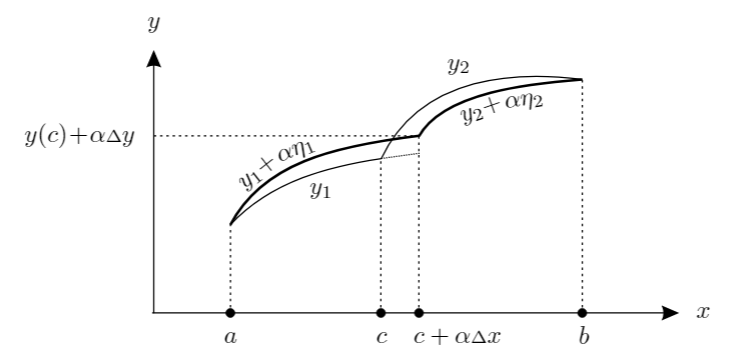
\includegraphics[width=0.95\textwidth]{img/extremalwtcorner.png}
        	\caption{A perturbation of a extremal with a corner (Liberzon p 73)}
        	% \label{}
        \end{figure}
    \end{frame}
    \begin{frame}
        Clearly from the previous figure and from the definition, \(y_1,y_2\) are only defined on disjoint segments of \(\left[a,b\right]\).\\\medskip
        We need to define continuations of these functions.\\
        For instance $y_1(x)$ all $x > c$ can be extended as $y_1(x) \defeq y(x) + y'(c^-)(x-c)$. Ditto for $y_2$. \\ \medskip
    \end{frame}
    \begin{frame}
        Now the functional to be optimized is given as
        \begin{equation*}
            \begin{split}
                 J ( y ) &= \int _ { a } ^ { b } L \left( x , y ( x ) , y ^ { \prime } ( x ) \right) d x  \\
                  &= \int _ { a } ^ { c } L \left( x , y _ { 1 } ( x ) , y _ { 1 } ^ { \prime } ( x ) \right) d x + \int _ { c } ^ { b } L \left( x , y _ { 2 } ( x ) , y _ { 2 } ^ { \prime } ( x ) \right) d x \\
                 &\defeq J _ { 1 } \left( y _ { 1 } \right) + J _ { 2 } \left( y _ { 2 } \right)
            \end{split}
        \end{equation*}
    \end{frame}
    \begin{frame}
        Let's look at the two terms separately.\\
        First
        \begin{equation*}
            J _ { 1 } \left( y _ { 1 } + \alpha \eta _ { 1 } \right) = \int _ { a } ^ { c + \alpha \Delta x } L \left( x , y _ { 1 } ( x ) + \alpha \eta _ { 1 } ( x ) , y _ { 1 } ^ { \prime } ( x ) + \alpha \eta _ { 1 } ^ { \prime } ( x ) \right) d x
        \end{equation*}
        which has an the following variation
        \begin{equation*}
            \begin{aligned} \delta J _ { 1 | y _ { 1 } } \left( \eta _ { 1 } \right) & = \left. \frac { d } { d \alpha } \right| _ { \alpha = 0 } J _ { 1 } \left( y _ { 1 } + \alpha \eta _ { 1 } \right) \\
                & = \int _ { a } ^ { c }  L _ { y } \left( x , y _ { 1 } ( x ) , y _ { 1 } ^ { \prime } ( x ) \right) \eta _ { 1 } ( x ) \\
                &+ L _ { y ^ { \prime } } \left( x , y _ { 1 } ( x ) , y _ { 1 } ^ { \prime } ( x ) \right) \eta _ { 1 } ^ { \prime } ( x )  d x  + L \left( c , y _ { 1 } ( c ) , y _ { 1 } ^ { \prime } ( c ) \right) \Delta x
            \end{aligned}
        \end{equation*}
    \end{frame}
    \begin{frame}
        \begin{equation*}
            \begin{split}
                \delta \left. J _ { 1 } \right| _ { y _ { 1 } } \left( \eta _ { 1 } \right) = \int _ { a } ^ { c } L _ { y } \left( x , y _ { 1 } ( x ) , y _ { 1 } ^ { \prime } ( x ) \right) \eta _ { 1 } ( x ) - \\
                - \frac { d } { d x } L _ { y ^ { \prime } } \left( x , y _ { 1 } ( x ) , y _ { 1 } ^ { \prime } ( x ) \right) \eta _ { 1 } ( x ) d x\\
                + L _ { y ^ { \prime } } \left( c , y ( c ) , y ^ { \prime } \left( c ^ { - } \right) \right) \eta _ { 1 } ( c )\\
                + L \left( c , y ( c ) , y ^ { \prime } \left( c ^ { - } \right) \right) \Delta x
            \end{split}
        \end{equation*}
        Same derivation follows through for \(\delta J_2\vert_{y_2}(\eta_2)\)
    \end{frame}
    \begin{frame}
        For sufficiently small $\alpha$ \(y(\cdot,\alpha)\) is close to $y(\cdot)$ in the 0-norm sense and so $J(y(\cdot,\alpha))$ attains a minimum at $\alpha=0$ which in turn implies that
        \begin{equation*}
            \delta \left. J _ { 1 } \right| _ { y _ { 1 } } \left( \eta _ { 1 } \right) + \delta \left. J _ { 2 } \right| _ { y _ { 2 } } \left( \eta _ { 2 } \right) = 0
        \end{equation*}
        which is equivalent to
        \begin{equation*}
            \begin{split}
                L _ { y ^ { \prime } } \left( c , y ( c ) , y ^ { \prime } \left( c ^ { - } \right) \right) \eta _ { 1 } ( c ) - L _ { y ^ { \prime } } \left( c , y ( c ) , y ^ { \prime } \left( c ^ { + } \right) \right) \eta _ { 2 } ( c )\\
                + L \left( c , y ( c ) , y ^ { \prime } \left( c ^ { - } \right) \right) \Delta x - L \left( c , y ( c ) , y ^ { \prime } \left( c ^ { + } \right) \right) \Delta x = 0
            \end{split}
        \end{equation*}
    \end{frame}
    \begin{frame}
        Now we show that the Lagrangian of the perturbed curve $y$ is continuous at $x = c + \alpha \Delta x$
        \begin{equation*}
            \begin{split}
                y _ { 1 } ( c + \alpha \Delta x ) + \alpha \eta _ { 1 } ( c + \alpha \Delta x ) = y _ { 2 } ( c + \alpha \Delta x ) + \alpha \eta _ { 2 } ( c + \alpha \Delta x ) \defeq \\                 \defeq y(c) + \alpha \Delta y + o(\alpha)
            \end{split}
        \end{equation*}
        which is a constant $y(c)$ plus first-order terms in $\alpha$. We equate the first oder terms
        \begin{equation*}
        y ^ { \prime } \left( c ^ { - } \right) \Delta x + \eta _ { 1 } ( c ) = y ^ { \prime } \left( c ^ { + } \right) \Delta x + \eta _ { 2 } ( c ) = \Delta y
        \end{equation*}
    \end{frame}

    \begin{frame}
        \begin{figure}[!htb]
            \centering
            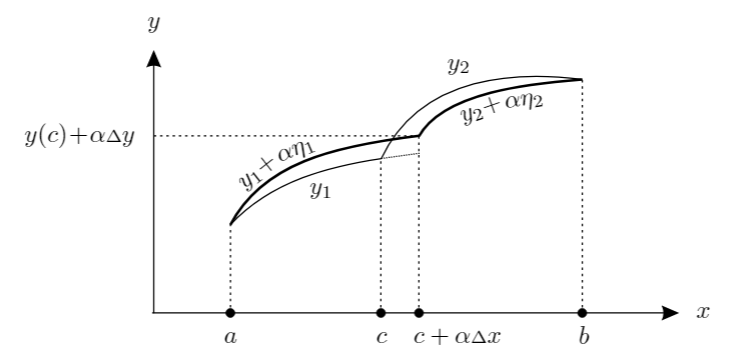
\includegraphics[width=0.95\textwidth]{img/extremalwtcorner.png}
            \caption{A perturbation of a extremal with a corner (Liberzon p 73)}
            % \label{}
        \end{figure}
    \end{frame}

    \begin{frame}
        Using the fact that the terms are
        \begin{figure}[!htb]
        	\centering
        	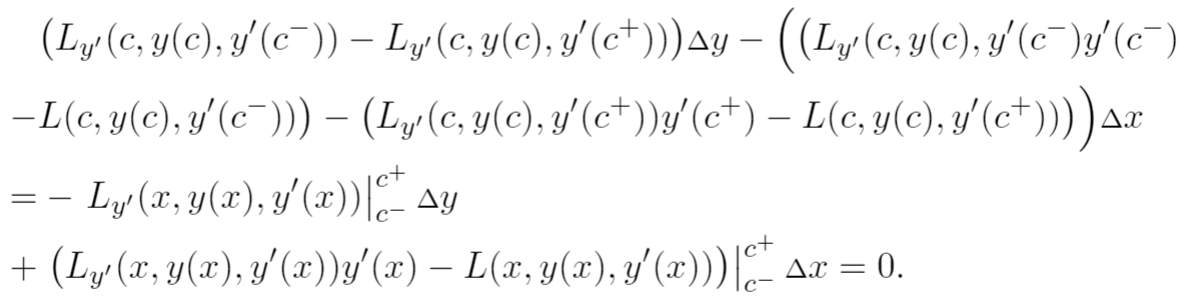
\includegraphics[width=0.95\textwidth]{ch3/WEcorner.png}
        	% \caption{}
        	% \label{}
        \end{figure}
        $\Delta x $ and $\Delta y$ are independent and arbitrary so this can only hold if the Lagrangian terms multiplying them are zero and the Lagrangian is continuous at $x = c + \alpha \Delta x$.
        \begin{theorem}{Weierstrass-Erdmann condition}
            If $y$ is a strong extremum then $L_{y^\prime}$ and $y^{\prime}L_{y^\prime} - L$ must be continuous at each corner point
        \end{theorem}
    \end{frame}

    \begin{frame}{Further conditions for strong optima}
        We consider a first order Taylor expansion of the Lagrangian around a curve $w$
        \begin{definition}[Weierstrass excess function]
            \begin{equation*}
                E ( x , y , z , w ) : = L ( x , y , w ) - L ( x , y , z ) - ( w - z ) \cdot L _ { z } ( x , y , z )
            \end{equation*}
        \end{definition}
        The \emph{Weierstrass necessary condition for a strong minimum}  states
        that if $y ( \cdot )$ is a strong minimum, then
        \begin{equation*}
        E \left( x , y ( x ) , y ^ { \prime } ( x ) , w \right) \geq 0
        \end{equation*}
        for all noncorner points $x \in [ a , b ]$ and all $w \in \mathbb { R }$
    \end{frame}
    \begin{frame}
        \begin{figure}[!htb]
            \centering
            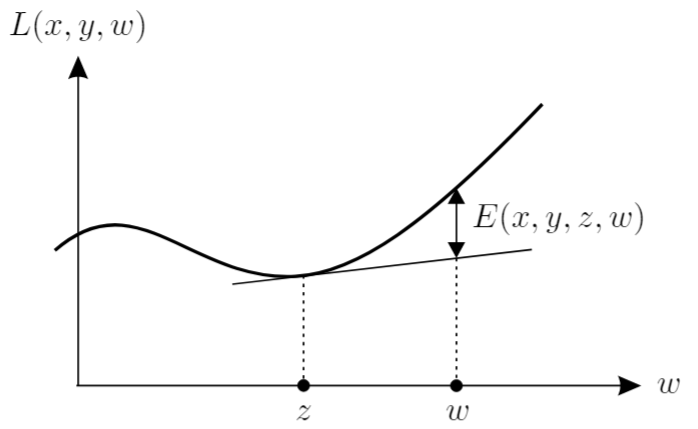
\includegraphics[width=0.95\textwidth]{ch3/Wexcess1.png}
            \caption{Weierstrass excess function. A measure of local stationarity, analogous to f.d. optim.}
            % \label{}
        \end{figure}
    \end{frame}
    \begin{frame}{Proof of the Weierstrass Excess function}
        Define a perturbation as
        \scalebox{0.83}{
            $y ( x , \varepsilon ) : = \left\{ \begin{array} { l l } { y ( x ) } & { \text { if } a \leq x \leq \overline { x } \text { or } d \leq x \leq b } \\ { y ( \overline { x } ) + w ( x - \overline { x } ) } & { \text { if } \overline { x } \leq x \leq \overline { x } + \varepsilon } \\ { y ( x ) + \frac { d - x } { d - ( \overline { x } + \varepsilon ) } ( y ( \overline { x } ) + w \varepsilon - y ( \overline { x } + \varepsilon ) ) } & { \text { if } \overline { x } + \varepsilon \leq x \leq d } \end{array} \right.$
        }
    \end{frame}
    \begin{frame}
        \begin{figure}[!htb]
	\centering
	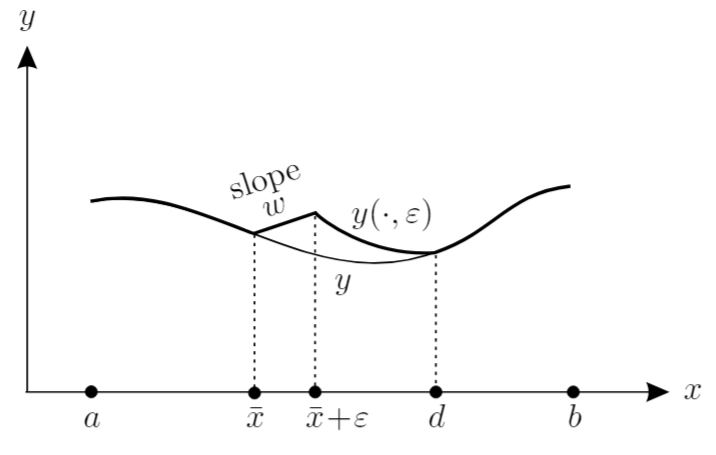
\includegraphics[width=0.95\textwidth]{ch3/Wexcess2.png}
	\caption{$y$ and $y(\cdot, \varepsilon)$}
	% \label{}
    \end{figure}
    \end{frame}
    \begin{frame}
        $\begin{aligned} \frac { d } { d \varepsilon } J ( y ( \cdot , \varepsilon ) ) = \frac { d } { d \varepsilon } & \left( \int _ { \overline { x } } ^ { \overline { x } + \varepsilon } L \left( x , y ( x , \varepsilon ) , y _ { x } ( x , \varepsilon ) \right) d x \right.\\ & + \int _ { \overline { x } + \varepsilon } ^ { d } L \left( x , y ( x , \varepsilon ) , y _ { x } ( x , \varepsilon ) \right) d x ) \end{aligned}$
        \\
        Clearly,
        $ \frac{d}{d\varepsilon} \int _ { \overline { x } } ^ { \overline { x } + \varepsilon } L ( x , y ( \overline { x } ) + w ( x - \overline { x } ) , w ) d x = L ( \overline { x } + \varepsilon , y ( \overline { x } ) + w \varepsilon , w )$
    \end{frame}
    \begin{frame}
        Similarly, the second term in variation of the functional $J$ is
        $ \frac{d}{d\varepsilon}
        \int _ { \overline { x } + \varepsilon } ^ { d } L \left( x , y ( x , \varepsilon ) , y _ { x } ( x , \varepsilon ) \right) d x
        $\\
        which equals\\
        \begin{figure}[!htb]
	\centering
	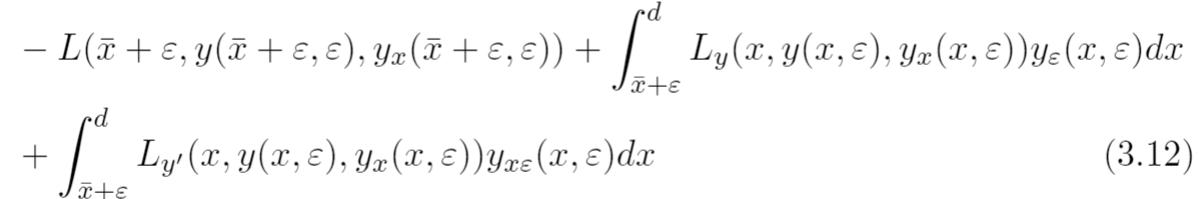
\includegraphics[width=0.95\textwidth]{ch3/Eq312.png}
	% \caption{}
	% \label{}
    \end{figure}
    \end{frame}
    \begin{frame}
        \begin{figure}[!htb]
	\centering
	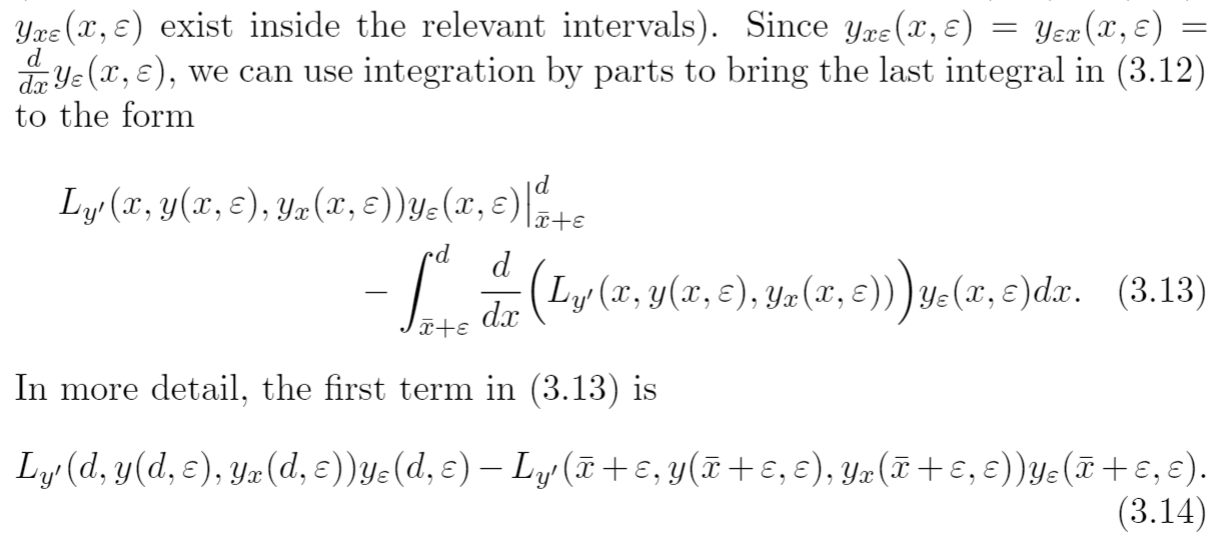
\includegraphics[width=0.95\textwidth]{ch3/Eq313314.png}
	% \caption{}
	% \label{}
    \end{figure}
    \end{frame}
    \begin{frame}
        \begin{figure}[!htb]
	\centering
	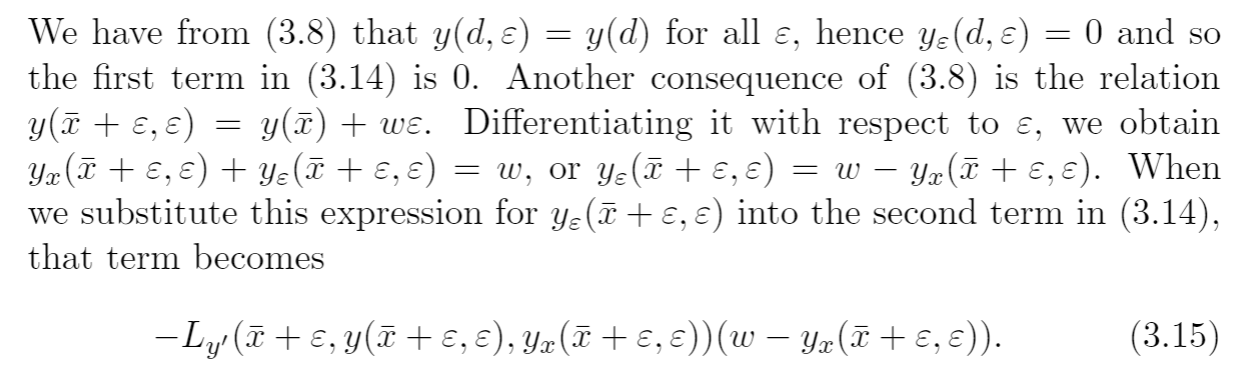
\includegraphics[width=0.95\textwidth]{ch3/Eq315.png}
	% \caption{}
	% \label{}
    \end{figure}
    \end{frame}
    \begin{frame}
        \begin{figure}[!htb]
	\centering
	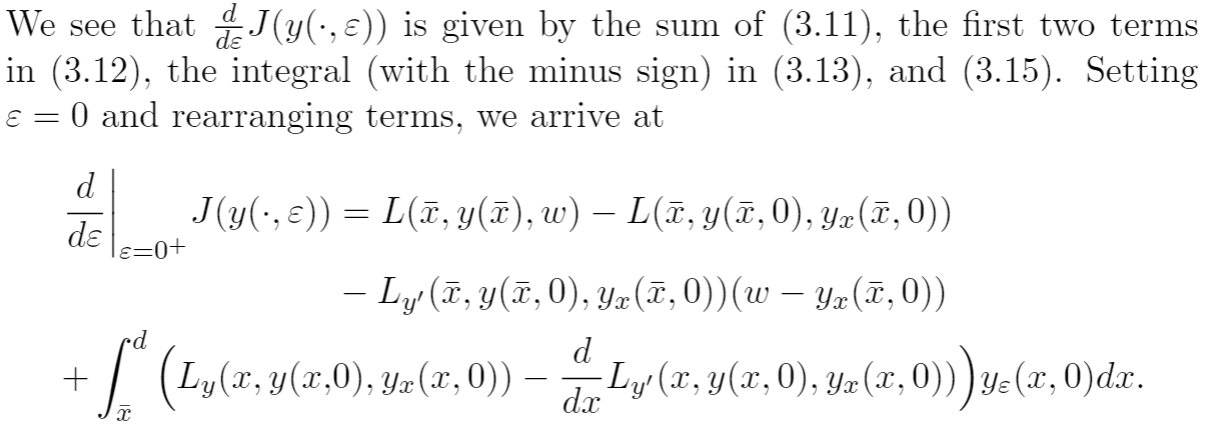
\includegraphics[width=0.95\textwidth]{ch3/Eq315b.png}
    	% \caption{}
    	% \label{}
    \end{figure}
    \end{frame}
    \begin{frame}
        \begin{figure}[!htb]
	\centering
	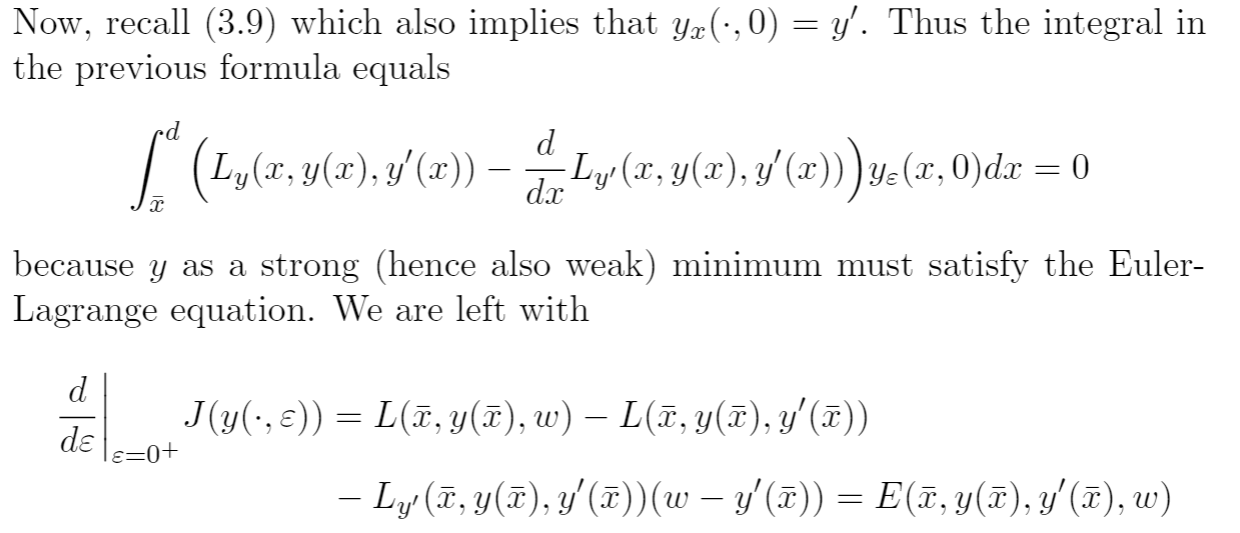
\includegraphics[width=0.95\textwidth]{ch3/Eq315c.png}
	% \caption{}
	% \label{}
    \end{figure}
    \end{frame}
    \begin{frame}
        Importantly we did not require the differentiability of $y$, but only used that $L$ be differentiable wrt. $y \textrm{and} y^{\prime}$.\\\medskip
        Finally, let's see how this relates to the Hamiltonian maximization conditions from before. Let's write the Hamiltonian as
        \begin{equation*}
            H ( x , y , z , p ) = z p - L ( x , y , z )
        \end{equation*}
        \begin{figure}[!htb]
	\centering
	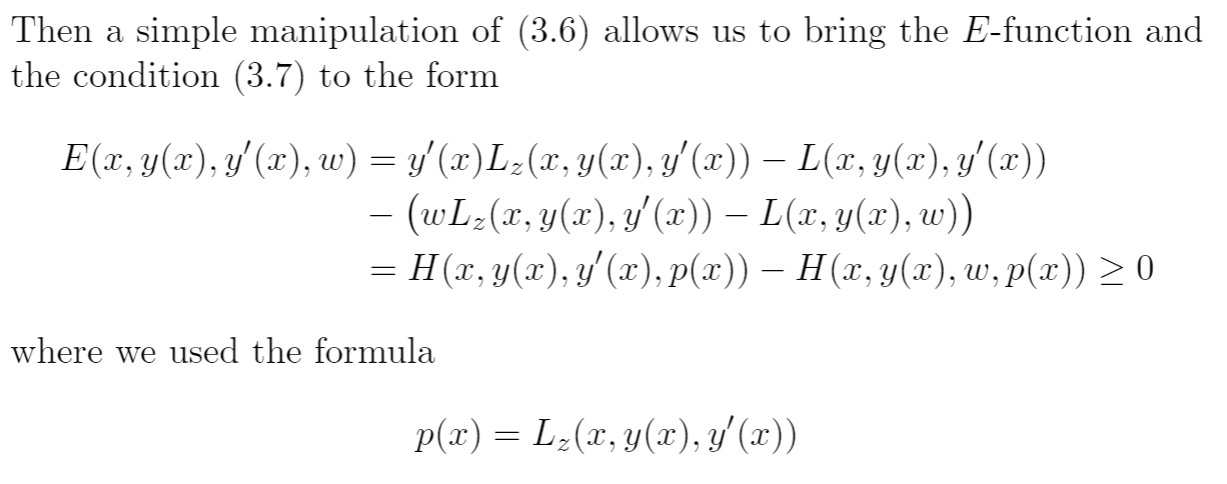
\includegraphics[width=0.95\textwidth]{ch3/HamiltonianThing.png}
	% \caption{}
	% \label{}
    \end{figure}
    \end{frame}
    \begin{frame}{Finally, control!}
        \begin{figure}[!htb]
	\centering
	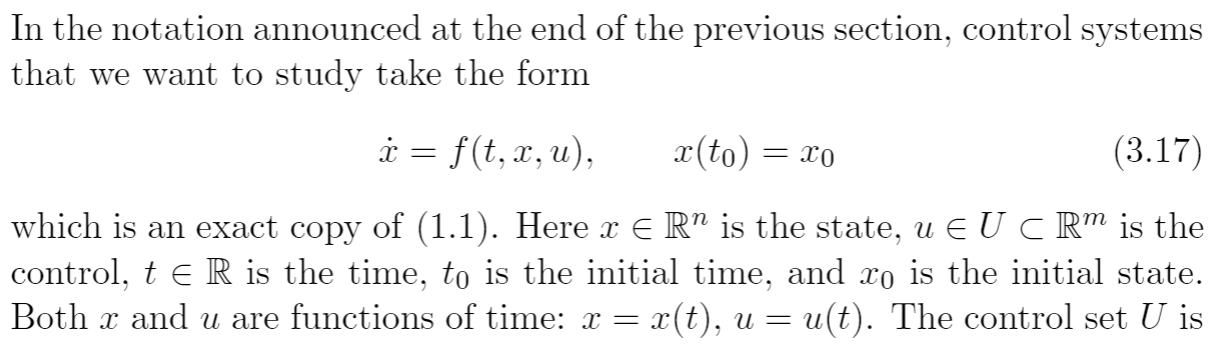
\includegraphics[width=0.95\textwidth]{ch3/ControlDef.png}
	% \caption{}
	% \label{}
    \end{figure}
    \end{frame}
    \begin{frame}{Cost functional}
        \begin{figure}[!htb]
	\centering
	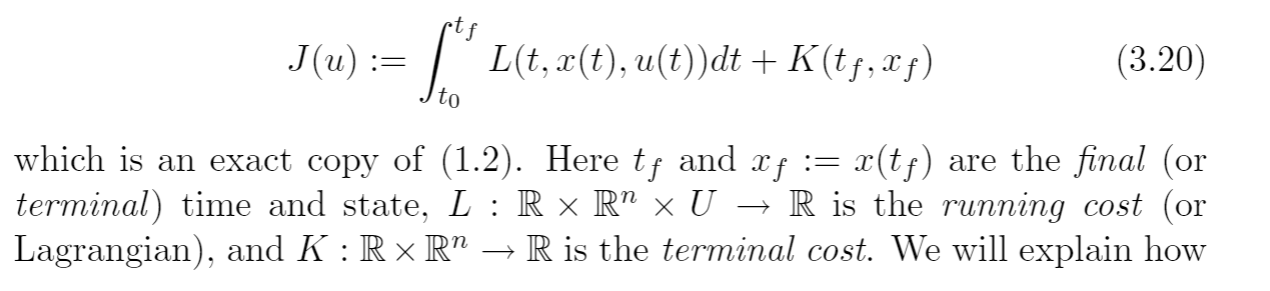
\includegraphics[width=0.95\textwidth]{ch3/CostFunctional.png}
	% \caption{}
	% \label{}
    \end{figure}
    \end{frame}
    \begin{frame}
        \begin{figure}[!htb]
	\centering
	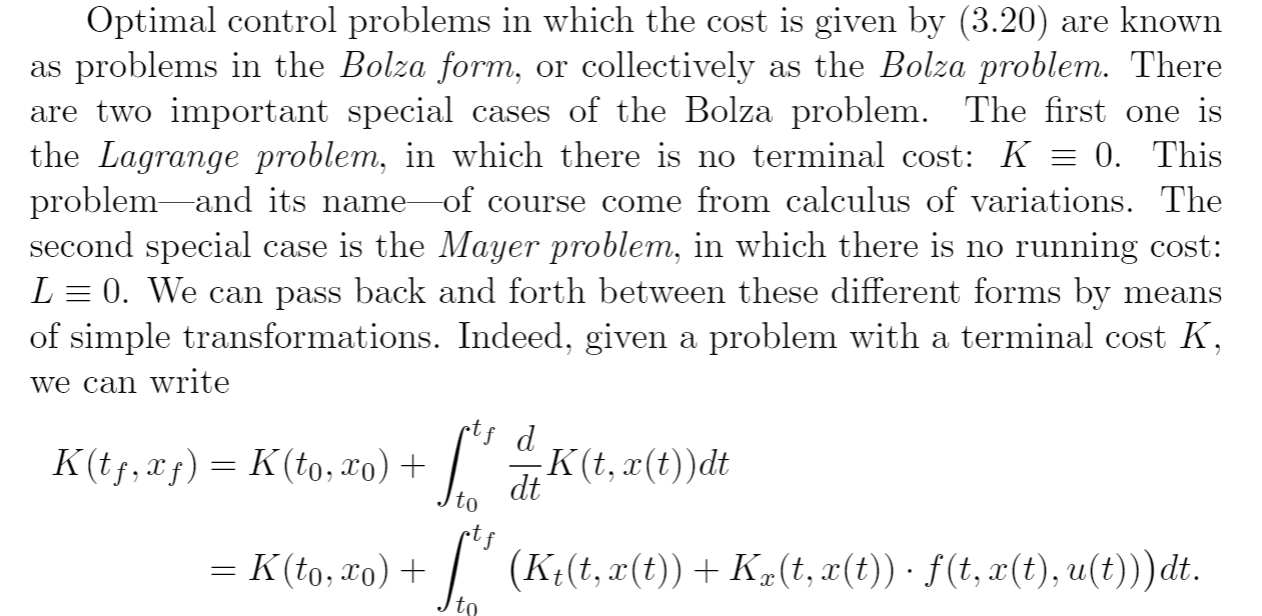
\includegraphics[width=0.95\textwidth]{ch3/Cost2.png}
	% \caption{}
	% \label{}
    \end{figure}
    \end{frame}
\end{document}
